\documentclass[11pt,a4paper]{article}

%\includeonly{05_reconstruction_two_views}

\usepackage[margin={2cm,2cm}]{geometry}
\setlength{\columnsep}{1cm}
\setlength{\parindent}{0pt}

\usepackage{graphics}
\usepackage{caption} % to use \caption*
\usepackage{mymaths}
\usepackage{mytext}
\usepackage{booktabs} % For formal tables
\usepackage{makecell} % Line break in cell

\begin{document}

\title{Multiple View Geometry}
\author{Course by Daniel Cremers --- transcript by Matthieu Pizenberg}
\date{June 2017}

\maketitle

\setcounter{tocdepth}{2}
\tableofcontents
\clearpage

\twocolumn
\section[Linear Algebra]{Mathematical Background: Linear Algebra}
\label{sec:linear_algebra}

This is intended as being a short crash course of linear algebra.

\subsection{Vector Spaces}
\label{sub:vector_spaces}

A set $V$ is called a \textbf{linear space}
or a \textbf{vector space over the field} $\R$
if it is closed under vector summation and scalar multiplication.
\begin{align*}
	+ &: V \times V \rightarrow V \\
	\cdot &: \R \times V \rightarrow V 
\end{align*}

\noindent
With respect to addition ($+$) it forms a commutative group
(existence of neutral element $0$, inverse element $-v$).
Scalar multiplication respects the structure of $\R$ 
($\alpha(\beta v) = (\alpha \beta )v$).
Multiplication and addition respect the \textbf{distributive law}:
\begin{align*}
	( \alpha + \beta )v &= \alpha v + \beta v \\
	\alpha (u + v) & = \alpha u + \alpha v
\end{align*}

\noindent
A subset $W \subset V$ of a vector space $V$
is called a \textbf{subspace} if $0 \in W$ and
$W$ is closed under $+$ and $\cdot$ (for all $\alpha \in \R$).\\

\noindent
A \textbf{spanned subspace} of a set of vectors
$S = \{v_1, \hdots, v_k\} \subset V$ is the subspace
formed by all linear combinations of these vectors.
The set $S$ is called \textbf{linearly independant} if:
\[
	\sum_{i=1}^k \alpha_i v_i = 0 \implies \forall i, \alpha_i = 0
\]
\noindent
A set $B = \{v_1, \hdots, v_n\}$ is called
a \textbf{basis} of $V$ if it is linearly independent and if it
spans the vector space $V$.
A basis is a maximal set of linearly independent vectors.


\subsubsection{Properties of a Basis}
\label{ssub:properties_of_a_basis}

Let $B$ and $B'$ be two bases of a linear space $V$.

\begin{enumerate}
	\item $B$ and $B'$ contain the same number of vectors.
	This number $n$ is called the \textbf{dimension of the space} $V$.

\item Any vector $v \in V$ can be \textbf{uniquely expressed}
	as a linear combination of the basis vectors in
	$B = \{b_1, \hdots, b_n\}$:
	\[
		v = \sum_{i=1}^n \alpha_i b_i
	\]
	\item In particular, all vectors of $B'$ can be expressed as
	linear combinations of vectors of $B$:
	\[
		b'_j = \sum_{i=1}^n \alpha_{ij} b_i
	\]
	The coefficients $\alpha_{ij}$ for this \textbf{basis transform}
	can be combined in a matrix $A$:
	\[
		B' = BA \Leftrightarrow B = B'A^{-1}
	\]
\end{enumerate}


\subsubsection{Inner Product}
\label{ssub:inner_product}

On a vector space, one can define an \textbf{inner product}
(or \textbf{dot product}):
\[\inner{\cdot}{\cdot} : V \times V \rightarrow \R\]
wich is defined by three properties:
\begin{enumerate}
	\item \textbf{linear}:
		$\inner{u}{\alpha v + \beta w} = \alpha \inner{u}{v} + \beta \inner{u}{w}$

	\item \textbf{symmetric}:
		$\inner{u}{v} = \inner{v}{u}$

	\item \textbf{positive definite}:\\
		$\inner{v}{v} \geq 0$ and $\inner{v}{v} = 0 \Leftrightarrow v = 0$
	
\end{enumerate}

\noindent
The scalar product induces a \textbf{norm}:
\[|\cdot| : V \rightarrow \R, \quad |v| = \sqrt{\inner{v}{v}}\]

\noindent
and a \textbf{metric}:
\[d : V \times V \rightarrow \R, \quad d(v,w) = |v - w| = \sqrt{\inner{v-w}{v-w}}\]

\noindent
A vector space with an inner product is then also
a \textbf{metric space}. It is called a \textbf{Hilbert space}.


\subsubsection{Canonical and Induced Inner Product}
\label{ssub:canonical_and_induced_inner_product}

On $V = \R^n$, one can define the canonical inner product for
the canonical basis $B = I_n$ as:

\[\inner{x}{y} = x^{\top} y = \sum_{i=1}^n x_i y_i\]

\noindent
which induces the standard $L_2$-norm or Euclidean norm:

\[|x|_2 = \sqrt{x^{\top}x} = \sqrt{x_1^2 + \hdots + x_n^2}\]

\noindent
With a basis transform $A$ to the new basis $B'$ given by
$B' = IA$ the canonical inner product in the new coordinates
$x'$, $y'$ is given by:

\[\inner{x}{y} = x^{\top} y = {(Ax')}^{\top} (Ay')
= x'^{\top} A^{\top} Ay' \equiv \inner{x'}{y'}_{A^{\top} A}\]

\noindent
The latter product is called the \textbf{induced inner product}
from the matrix $A$.\\

\noindent
Two vectors $v$ and $w$ are \textbf{orthogonal} iff\\
$\inner{v}{w} = 0$.


\subsubsection{Kronecker Product and Stack of a Matrix}
\label{ssub:kronecker_product_and_stack_of_a_matrix}

Given two matrices $A \in \R^{m\times n}$ and $B \in \R^{k \times l}$,
one can define their \textbf{Kronecker product} by:

\[A \otimes B \equiv
	\begin{pmatrix}
		a_{11}B & \cdots & a_{1n}B \\
		\vdots & \ddots & \vdots \\
		a_{m1}B & \cdots & a_{mn}B \\
	\end{pmatrix}
\]
\noindent
In matlab: $C = \mathrm{kron}(A,B)$.

\noindent
Given a matrix $A \in \R^{m \times n}$, its \textbf{stack} $A^s$
is obtained by stacking its $n$ column vectors $a_1, \ldots, a_n \in \R^m$:

\[A^s \equiv
	\begin{pmatrix}
		a_1 \\
		\vdots \\
		a_n \\
	\end{pmatrix}
\in \R^{mn}\]

\noindent
These notations allow to rewrite algebraic expressions, for example:

\[u^{\top} A v = {( v \otimes u )}^{\top} A^s\]

\subsection{Linear Transformations and Matrices}
\label{sub:linear_transformations_and_matrices}

A \textbf{linear transformation} $L$ between tow linear spaces
$V$ and $W$ is a map $L : V \rightarrow W$ such that:
\begin{align*}
	\forall (x,y) \in V^2 ,\quad L(x+y) &= L(x) + L(y) \\
	\forall x \in V, \forall \alpha \in \R,\quad L(\alpha x) &= \alpha L(x)
\end{align*}

\noindent
Due to the linearity, the action of $L$ on the space $V$
is uniquely defined by its action on the basis vectors of $V$.
In the canonical basis ${e_1, \ldots, e_n}$ we have:

\[\forall x \in V, \quad L(x) = Ax\]
\noindent
where
\[A = (L(e_1), \ldots, L(e_n)) \in \R^{m \times n}\]

\noindent
The set of all $m \times n$ matrices is denoted by $\M(m,n)$.
In case that $m = n$, the set $\M(m,n) \equiv \M(n)$
forms a \textbf{ring} over the field $\R$, i.e.\ it is closed
under matrix multiplication and summation.


\subsubsection{The Linear Groups $GL(n)$ and $SL(n)$}
\label{ssub:the_linear_groups_gl_n_and_sl_n_}

A \textbf{group} is a set $G$ with an operation
$\circ : G \times G \rightarrow G$ such that:
\begin{enumerate}
	\item It is closed:
		$\forall (g_1, g_2) \in G^2, \quad g_1 \circ g_2 \in G$
	\item It is associative:
		$\forall (g_1, g_2, g_3) \in G^3, \quad
		(g_1 \circ g2) \circ g_3 = g_1 \circ (g_2 \circ g_3)$
	\item There is a neutral element:
		$\exists e \in G: \forall g \in G, \quad
		e \circ g = g \circ e = g$
	\item Each element has an inverse:
		$\forall g \in G, \exists \inv{g} \in G : \quad
		g \circ \inv{g} = \inv{g} \circ g = e$
\end{enumerate}

\noindent
All invertible (non-singular) real $n \times n$ matrices
form a group with respect to matrix multiplication.
This group is called the \textbf{general linear group} $GL(n)$.
It consists of all $A \in \M(n)$ for which $\det(A) \ne 0$.\\

\noindent
All matrices $A \in GL(n)$ for which $\det(A) = 1$ form a group
called the \textbf{special linear group} $SL(n)$.


\subsubsection{Matrix Representation of Groups}
\label{ssub:matrix_representation_of_groups}

A group $G$ has a \textbf{matrix representation} or can be realized as
a matrix group if there exists an injective transformation:

\[R : G \rightarrow GL(n)\]

\noindent
which \textbf{preserves the group structure} of $G$,
that is inverse and composition are preserved by the map:

\begin{align*}
	R(e) &= I_{n \times n} \\
	\forall (g,h) \in G^2, \quad R(g\circ h) &= R(g)R(h)
\end{align*}

\noindent
Such a map $R$ is called a \textbf{group homomorphism}.
The idea is to study properties of the group by the matrices properties.


\subsubsection{The Affine Group $A(n)$}
\label{ssub:the_affine_group_a_n_}

An affine transformation $L : \R^n \rightarrow \R^n$
is defined by a matrix $A \in GL(n)$ and a vector $b \in \R^n$ such that:
\[L(x) = Ax + b\]

\noindent
The set of all such affine transformations is called the
\textbf{affine group of dimension $n$}, denoted by $A(n)$.
L defined above is not a linear map unless $b=0$.
By introducing \textbf{homogeneous coordinates} to represent $x \in \R^n$ by
$\inmatrix{x \\ 1} \in \R^{n+1}$,
$L$ becomes a linear mapping from:

\[L: \R^{n+1} \rightarrow \R^{n+1}; \quad
	\begin{pmatrix}
		x \\
		1 \\
	\end{pmatrix}
	\mapsto
	\begin{pmatrix}
		A & b \\
		0 & 1 \\
	\end{pmatrix}
	\begin{pmatrix}
		x \\
		1 \\
	\end{pmatrix}\]

\noindent
A matrix $\inmatrix{A & b \\ 0 & 1}$ with $A \in GL(n)$ and $b \in R^n$
is called an \textbf{affine matrix}. It is an element of $GL(n+1)$.
The affine matrices form a subgroup of $GL(n+1)$.


\subsubsection{The Orthogonal Group $O(n)$}
\label{ssub:the_orthogonal_group_o_n_}

A matrix $A \in \M(n)$ is called \textbf{orthogonal} if it preserves
the inner product:
\[\forall (x,y) \in {(\R^n)}^2 \quad \inner{Ax}{Ay} = \inner{x}{y}\]

\noindent
The set of all orthogonal matrices forms the \textbf{orthogonal group}
$O(n)$, which is a subgroup of $GL(n)$.
For an orthogonal matrix $R$ we have:
\[\forall (x,y) \in {(\R^n)}^2, \quad
\inner{Rx}{Ry} = \tr{x}\tr{R}Ry = \tr{x}y\]

\noindent
Therefore, we must have $\tr{R}R = R\tr{R} = I$, i.e.
\[O(n) = \{ R \in GL(n) \ | \ \tr{R}R = I \}\]

\noindent
We can show that $\det(R) \in \{ \pm 1\}$.
The subgroup of $O(n)$ with $\det(R) = +1$ is called
the \textbf{special orthogonal group} $SO(n)$.
$SO(n) = O(n) \cap SL(n)$.
In particular, $SO(3)$ is the group of all 3-dimensional rotation matrices.


\subsubsection{The Euclidean Group $E(n)$}
\label{ssub:the_euclidean_group_e_n_}

A Euclidean transformation $L$ from $\R^n$ to $\R^n$ is defined by
an orthogonal matrix $R \in O(n)$ and a vector $T \in R^n$:
\[L : \R^n \rightarrow \R^n; \quad x \mapsto Rx + T\]

\noindent
The set of all such transformations is called the
\textbf{Euclidean group} $E(n)$. It is a subgroup of the affine group $A(n)$.
\[E(n) = \left\{
	\begin{pmatrix}
		R & T \\
		0 & 1 \\
	\end{pmatrix}
\ \middle| \ R \in O(n), \ T \in \R^n \right\}\]


\noindent
If $R \in SO(n)$ then we have the \textbf{special euclidean group} $SE(n)$.
In particular, $SE(3)$ represent the \textbf{rigid-body motions} in $\R^3$.\\

\noindent
In summary:

\[\boxed{SO(n) \subset O(n) \subset GL(n)}\]
\[\boxed{SE(n) \subset E(n) \subset A(n) \subset GL(n+1)}\]


\subsection{Properties of Matrices}
\label{sub:properties_of_matrices}


\subsubsection{Range, Span, Null Space and Kernel}
\label{ssub:range_span_null_space_and_kernel}

Let $A \in \Rmn$ be a matrix defining a linear map from $\Rn$ to $\Rm$.
The \textbf{range} or \textbf{span} of $A$ is defined as the subspace
of $\Rm$ which can be ``reached'' by $A$:
\[\text{range}(A) = \{ y \in \Rm \ |\  \exists x \in \Rn : Ax = y \}\]

\noindent
The range of a matrix $A$ is given by the span of its column vectors.
The \textbf{null space} or \textbf{kernel} of a matrix $A$ is given by
the subset of vectors $x \in \Rn$ which are mapped to zero:
\[\text{null}(A) \equiv \ker(A) = \{ x \in \Rn \ | \ Ax = 0 \}\]

\noindent
The null space of a matrix $A$ is given by the vectors
orthogonal to its row vectors. In matlab: $Z = \text{null}(A)$.
The concepts of range and null space are useful when studying the
\textbf{solution of linear equations}. The system $Ax = b$ will have
a solution $x \in \Rn$ if and only if $b \in \text{range}(A)$.
Moreover, this solution will be unique only if $\ker(A) = \{0\}$.\\

\noindent
The \textbf{rank} of a matrix is the dimension of its range:
\[\text{rank}(A) = \dim(\text{range}(A))\]

\noindent
The rank of a matrix $A \in \Rmn$ has the following properties:
\begin{enumerate}
	\item $\text{rank}(A) = n - \dim(\ker(A))$
	\item $0 \le \text{rank}(A) \le \min\{m,n\}$.
	\item $\text{rank}(A)$ is equal to the maximum number
		of linearly independent row (or column) vectors of $A$.
	\item $\text{rank}(A)$ is the highest order of a nonzero minor of $A$,
		where a \textbf{minor of order k} is the determinant
		of a $k \times k$ submatrix of $A$.
	\item \textbf{Sylvester's inequality}: Let $B \in \R^{n \times k}$.
		then $AB \in \R^{m \times k}$ and
		$\text{rank}(A) + \text{rank}(B) - n \le
			\text{rank}(AB) \le \min \{ \text{rank}(A), \text{rank}(B)\}$.
	\item For any nonsingular matrices $C \in \R^{m \times m}$
		and $D \in \R^{n \times n}$, we have:
		$\text{rank}(A) = \text{rank}(CAD)$.
\end{enumerate}

\section{Representing a Moving Scene}%
\label{sec:moving_scene}


\subsection{The Origins of 3D Reconstruction}%
\label{sub:the_origins_of_3d_reconstruction}

The goal to reconstruct the three-dimensional structure of the world from
a set of two-dimensional views has long history in computer vision.
It is a classical \textbf{ill-posed problem}, because the reconstruction
consistent with a given set of observations/images is typically not unique.
Therefore, one will need to impose additional assumptions.
Mathematically, the study of geometric relations between a 3D scene
and the observed 2D projections is based on two types of transformations, namely:
\begin{itemize}
	\item \textbf{Euclidean motion} or \textbf{rigid body motion}
		representing the motion of the camera from one frame to the next.
	\item \textbf{Perspective projection} to account for the image formation
		process (see pinhole camera, etc).
\end{itemize}

The notion of perspective projection has its roots among the ancient Greeks
(Euclid of Alexandria, \roughly{} 400 B.C.) and the Renaissance period
(Brunelleschi \& Alberti, 1435).
The study of perspective projection lead to the field of
\textbf{projective geometry} (Girard Desargues 1648, Gaspard Monge 18th cent).\\

The first work on the problem of multiple view geometry was that of
\textbf{Erwin Kruppa (1913)} who showed that two views of five points
are sufficient to determine both the relative tansformation
(\textbf{motion}) between the two views and the 3D location (\textbf{structure})
of the points up to finitely many solutions.\\

A linear algorithm to recover structure and motion from two views based
on the epipolar constraint was proposed by \textbf{Longuet-Higgins}
in \textbf{1981}. An entire series of works along these lines was summarized
in several text books (Faugeras 1993, Kanatani 1993,
Maybank 1993, Weng et al. 1993).\\

Extensions to three views were developed by Spetsakis and Aloimonos '87, '90
, and by Shashua '94 and Hartley '95.
Factorization techniques for multiple views and orthogonal projection were
developed by Tomasi and Kanade 1992.\\

The joint estimation of camera motion and 3D location is called
\textbf{structure and motion} or \textbf{visual SLAM}.


\subsection{3D Space \& Rigid Body Motion}%
\label{sub:3d_space_rigid_body_motion}


\subsubsection{Three-dimensional Euclidean Space}%
\label{ssub:three_dimensional_euclidean_space}

The three-dimensional Euclidean space $\E^3$ consists of all points
$p \in \E^3$ characterized by coordinates
	\[\bm{X} \equiv \tr{(X_1, X_2, X_3)} \in \R^3\]

such that $\E^3$ can be identified with $\R^3$.
That means we talk about points ($\E^3$) and coordinates ($\R^3$)
as if they were the same thing. Given two points $\bm{X}$ and $\bm{Y}$,
one can define a \textbf{bound vector} as
	\[v = \bm{Y} - \bm{X} \in \R^3\]

Considering this vector independent of its base point $\bm{Y}$ makes
it a \textbf{free vector}. The set of free vectors $v \in \R^3$
forms a linear vector space. By identifying $\E^3$ and $\R^3$,
one can endow $\E^3$ with a scalar product, a norm and a metric.
This allows to compute \textbf{distances, curve length, areas or volumes.}
\[\text{For a curve } \gamma : [0,1] \rightarrow \R^3,\quad
	l(\gamma) \equiv \int_{0}^1 | \dot{\gamma}(s) | d\!s\]


\subsubsection{Cross Product \& Skew-symmetric Matrices}%
\label{ssub:cross_product_and_skew_symmetric_matrices}

On $\R^3$ one can define a cross product
\[\times : \R^3 \times \R^3 \rightarrow \R^3,\quad u \times v =
	\begin{pmatrix}
		u_2v_3 - u_3v_2 \\
		u_3v_1 - u_1v_3 \\
		u_1v_2 - u_2v_1
	\end{pmatrix} \in \R^3\]

which is a vector \textbf{orthogonal to $u$ and $v$}.
Since $u \times v = -v \times u$, the cross product introduces an \textbf{orientation}.
Fixing $u$ induces a linear mapping $v \mapsto u \times v$ wich
can be represented by the \textbf{skew-symmetric matrix}
\[\widehat{u} = \hatmat{u_1}{u_2}{u_3} \in \RR{3}{3}\]

In turn, every skew symmetric matrix $M = -\tr{M} \in \RR{3}{3}$
can be identified with a vector $u \in \R^3$.
The operator $\widehat{}$ defines an \textbf{isomorphism} between $\R³$
and the space $so(3)$ of the $3 \times 3$ skew-symmetric matrices.
Its inverse is denoted by $\vee : so(3) \rightarrow \R^3$.


\subsubsection{Rigid-body Motion}%
\label{ssub:rigid_body_motion}

A \textbf{rigid-body motion} (or rigid-body transformation)
is a family of maps
\[g_t : \R^3 \rightarrow \R^3;\quad \bm{X} \mapsto g_t(\bm{X}),\quad t \in [0,T]\]

which preserve the norm and cross product of any two vectors:
\begin{itemize}
	\setlength\itemsep{-0.2em}
	\item $\forall v \in \R^3, \quad |g_t(v)| = |v|$
	\item $\forall u,v \in \R^3, \quad g_t(u) \times g_t(v) = g_t(u \times v)$
\end{itemize}

Since norm and scalar product are related by the \textbf{polarization identity}
\[\inner{u}{v} = \frac{1}{4}(|u+v|^2 - |u-v|^2)\]

one can also state that a rigid-body motion is a map which
preserves inner product and cross product.
As a consequence, rigid-body motions also preserves the \textbf{triple product}
\[\forall u, v, w \in \R^3, \quad
	\inner{g_t(u)}{g_t(v) \times g_t(w)} = \inner{u}{v \times w}\]

which means that they are volume-preserving.


\subsubsection{Representation of Rigid-body Motion}%
\label{ssub:representation_of_rigid_body_motion}

Let $g_t$ our rigid body motion. We are going to detail what this transformation
is doing to the initial frame of orthonormal oriented vecors
$e_1, e_2, e_3 \in \R^3$.
We note the transformed vectors $r_i = g_t(e_i)$.
Scalar and cross product of these vectors are preserved:
	\[\tr{r_i}r_j = \tr{g_t(e_i)}g_t(e_j) = \tr{e_i}e_j = \delta_{ij}, \quad
	r_1 \times r_2 = r_3\]

The first constraint amounts to the statement that the matrix
$R = (r_1, r_2, r_3)$ is an orthogonal matrix: $\bm{\tr{R}R=R\tr{R}=I}$,
whereas the second property implies that $\bm{\det(R) = +1}$.
In other words: $R$ is an element of the group
$SO(3) = \{R \in \RR{3}{3}\ |\ \tr{R}R=I,\ \det(R) = +1\}$.\\

The motion of the origin can be represented by a \textbf{translation}
$\bm{T \in R^3}$. Thus the rigid body motion $g_t$ can be written as:
	\[g_t(x) = Rx + T\]


\subsubsection{Exponential Coordinates of Rotation}%
\label{ssub:exponential_coordinates_of_rotation}

We will now derive a representation of an \textbf{infinitesimal rotation}.
To this end, we consider a family of rotation matrices $R(t)$
which continuously transform a point from its original location
$(R(0) = I)$ to a different one.
	\[\bm{X}_{\text{trans}}(t) = R(t)\bm{X}_{\text{orig}}, \quad
	\text{with } R(t) \in SO(3)\]

Since $\forall t,\ R(t)\tr{R(t)} = I$, we have:
	\[\frac{d}{dt}(R\tr{R}) = \dot{R}\tr{R} + R\tr{\dot{R}}= 0
	\implies \dot{R}\tr{R} = -\tr{( \dot{R}\tr{R} )}\]

Thus, $\dot{R}\tr{R}$ is a \textbf{skew-symmetric matrix}.
As shown in the section about the $\widehat{}$ operator, this implies that
there exists a vector $w(t) \in \R^3$ such that:
	\[\dot{R}(t)\tr{R}(t) = \widehat{w}(t)
	\Leftrightarrow \bm{ \dot{R}(t) = \widehat{w}(t)R(t)}\]

Since $R(0) = I$, it follows that $\dot{R}(0) = \widehat{w}(0)$.
Therefore, the \textbf{skew-symmetric matrix $\bm{\widehat{w}(0) \in so(3)}$
gives the first order approximation of a rotation:}
	\[R(dt) = R(0) + dR = I + \widehat{w}(0) dt\]


\subsection{The Lie Group $SO(3)$}%
\label{sub:the_lie_group_so_3_}


\subsubsection{Lie Group and Lie Algebra}%
\label{ssub:lie_group_and_lie_algebra}

The above calculations showed that the effect of any infinitesimal
rotation $R \in SO(3)$ can be approximated by an element from
the space of skew-symmetric matrices
	\[so(3) = \{ \widehat{w}\ |\ w \in \R^3\}\]

The rotation group $SO(3)$ is called a \textbf{Lie group}.
The space $so(3)$ is called its \textbf{Lie algebra}.\\

\underline{Definition:}
A \textbf{Lie group} (or infinitesimal group) is a smooth manifold that
is also a group, such that the group operations multiplication
and inversion are smooth maps.\\

As shown above: \textbf{The Lie algebra $\bm{so(3)}$ is the tangent space
at the identity of the rotation group $\bm{SO(3)}$.}\\

An \textbf{algebra over a field $\bm{K}$} is a vector space $V$ over $K$
with multiplication on the space $V$.
Elements $\widehat{w}$ and $\widehat{v}$ of the Lie algebra
generally do not commute.
One can define the \textbf{Lie bracket}
\[[\cdot,\cdot]: so(3) \times so(3) \rightarrow so(3);\quad
[\widehat{w},\widehat{v}] \equiv \widehat{w}\widehat{v} - \widehat{v}\widehat{w}\]


\subsubsection{Sophus Lie (1841--1899)}%
\label{ssub:sophus_lie_1841_1899_}

\begin{figure}[ht]
\centering
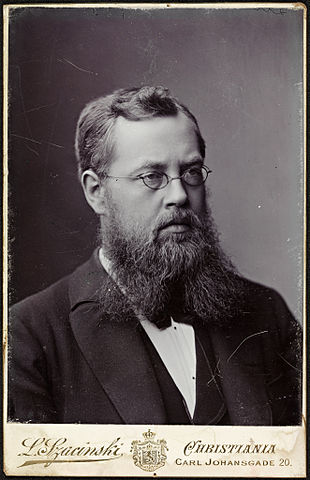
\includegraphics[width=10em]{img/sophus_lie.jpg}
\caption*{Portrait of Marius Sophus Lie}
\end{figure}

Marius Sophus Lie was a Norwegian-born mathematician.
He created the theory of \textbf{continuous symmetry}, and applied it to
the study of geometry and differential equations. Among his greatest
achievements was the discovery that continuous transformation
groups are better understood in their linearized versions
(``Theory of transformation groups'' 1893).
These \textbf{infinitesimal generators} form a structure which is today
known as a \textbf{Lie algebra}. The linearized version of the group law
corresponds to an operation on the Lie algebra known as
the \textbf{commutator bracket} or \textbf{Lie bracket}.
1882 Professor in Christiania (Oslo),
1886 Leipzig (succeeding Felix Klein),
1898 Christiania.


\subsubsection{The Exponential Map}%
\label{ssub:the_exponential_map}

Given the infinitesimal formulation of rotation,
we got to the differential equation system:
	\[\left\{ \begin{aligned}
		\dot{R}(t) &= \widehat{w}(t)R(t) \\
		R(0) &= I \\
	\end{aligned}\right.\]

If we assume that $\widehat{w}(t)$ is constant in time ($=\widehat{w}$),
this known equation has the solution:
	\[R(t) = e^{\widehat{w}t}
		= \sum_{n=0}^{\infty} \frac{{(\widehat{w}t)}^n }{n!}
		= I + \widehat{w}t + \frac{{(\widehat{w}t)}^2 }{2!} + \ldots \]

which is a rotation around the axis $w \in \R^3$
by an angle of t (if $\|w\| = 1$). Alternatively, one can absorb
the scalar $t \in \R$ into the skew  symmetric matrix $\widehat{w}$
to obtain $R(t) = e^{\widehat{v}}$ with $\widehat{v} = \widehat{w}t$.
This \textbf{matrix exponential} therefore defines a map from
the Lie algebra to the Lie group:
	\[\exp : so(3) \rightarrow SO(3);\quad \widehat{w}\mapsto e^{\widehat{w}}\]


\subsubsection{The Logarithm of $SO(3)$}%
\label{ssub:the_logarithm_of_so_3_}

There is conversely a mapping from the Lie group to the Lie algebra.
For any rotation matrix $R \in SO(3)$, there exists a $w \in \R^3$
such that $R = \exp(\widehat{w})$. Such an element is denoted by
$\widehat{w} = \log(R)$. If $R \ne I$, we note $r_{ij}$ its coefficients
and $w$ is given by:
	\[\left\{ \begin{aligned}
		|w| &= \inv{\cos}\left(\frac{\text{trace}(R)-1}{2}\right)\\
		\frac{w}{|w|} &= \frac{1}{2\sin(|w|)}
			\begin{pmatrix}
				r_{32} - r_{23} \\
				r_{13} - r_{31} \\
				r_{21} - r_{12} \\
			\end{pmatrix}
	\end{aligned}\right.\]

For $R = I$, we have $|w| = 0$, i.e.\ a rotation by an angle 0.
The above statement says:
\textbf{Any orthogonal transformation $\bm{\R \in SO(3)}$ can be realized
by rotating by an angle $\bm{|w|}$ around an axis
$\bm{\frac{w}{|w|}}$ as defined above}.\\

Obviously the above representation is not unique since for example,
increasing the angle by multiples of $2\pi$ will give the same rotation.


\subsubsection{Rodrigues' Formula}%
\label{ssub:rodrigues_formula}

In analogy to the well-known Euler equation
	\[\forall \phi \in \R, \quad  e^{i\phi} = \cos(\phi) + i\ \sin(\phi)\]

we have an expression for skew symmetric matrices $\widehat{w} \in so(3)$:
	\[\boxed{
	e^{\widehat{w}} = I + \frac{\widehat{w}}{|w|} \sin(|w|)
		+ \frac{\widehat{w}^2}{|w|^2} (1 - \cos(|w|))}\]

This is known as \textbf{Rodrigues' formula}.\\

\underline{Proof sketch:}
Let $t = |w|$ and $v = w/|w|$ such that $w = vt$. Then one can show that:
	\[\widehat{v}^2 = v\tr{v} - I \quad
	\text{and}\quad \widehat{v}^3 = -\widehat{v}\]
Thus, by developing the exponential, we get:
	\[e^{\widehat{v}t} = I +
		\underbrace{\left( t - \frac{t^3}{3!} + \cdots \right)}_{\sin(t)}\widehat{v}
	+ \underbrace{\left(\frac{t^2}{2!}-\frac{t^4}{4!}+\cdots \right)}_{1-\cos(t)}
		\widehat{v}^2\]


\subsection{The Lie Group $SE(3)$}%
\label{sub:the_lie_group_se_3_}


\subsubsection{Representation of Rigid-body Motions $SE(3)$}%
\label{ssub:representation_of_rigid_body_motions_se_3_}

We have seen that the space of rigid-body motions is given by
the group of special Euclidean transformations:
	\[SE(3) \equiv \{ g = (R,T)\ |\ R \in SO(3),\ T \in \R^3\}\]
In homogeneous coordinates:
	\[\boxed{SE(3) \equiv
	\left\{ g = \begin{pmatrix}
		R & T \\
		0 & 1 \\
	\end{pmatrix}\ \middle|\ R \in SO(3), T \in \R^3\right\}}\]

In the context of rigid motions, one can see the difference
between points in $\E^3$ (which can be rotated and translated)
and vectors in $\R^3$ (which can only be rotated).


\subsubsection{The Lie Algebra of Twists}%
\label{ssub:the_lie_algebra_of_twists}

Given a continuous family of rigid-body transformations:
	\[g : \R \rightarrow SE(3);\quad g(t) = \begin{pmatrix}
		R(t) & T(t) \\
		0 & 1 \\
	\end{pmatrix}\ \in \RR{4}{4}\]

we consider:
	\[\dot{g}(t)\inv{g}(t) = \begin{pmatrix}
		\dot{R}\tr{R} & \dot{T} - \dot{R}\tr{R}T \\
		0 & 0 \\
	\end{pmatrix}\ \in \RR{4}{4}\]

As in the case of $SO(3)$ the $\dot{R}\tr{R}$ corresponds
to some skew-symmetric matrix $\widehat{w} \in so(3)$. Defining a vector
$v(t) = \dot{T}(t) - \widehat{w}(t)T(t)$, we have:
	\[\dot{g}(t)\inv{g}(t) = \begin{pmatrix}
		\widehat{w}(t) & v(t) \\
		0 & 0 \\
	\end{pmatrix} \equiv \widehat{\xi}(t) \in \RR{4}{4}\]

Multiplying with $g(t)$ from the right, we obtain:
	\[\dot{g} = \dot{g}\inv{g}g = \widehat{\xi}g\]

The $4 \times 4$ matrix $\widehat{\xi}$ can be viewed as a tangent vector
along the curve $g(t)$. $\widehat{\xi}$ is called a \textbf{twist}.
As in the case of $so(3)$, the set of all twists forms the tangent
space which is the \textbf{Lie algebra}
	\[\boxed{se(3) \equiv \left\{ \widehat{\xi} = \begin{pmatrix}
		\widehat{w} & v \\
		0 & 0 \\
	\end{pmatrix}\ \middle|
	\ \widehat{w} \in so(3),\ v \in \R^3 \right\}}\]

	to the \textbf{Lie group $\bm{SE(3)}$}.\\

As before, we can define operators $\wedge$ and $\vee$ to convert between
a \textbf{twist $\bm{\widehat{\xi} \in se(3)}$} and its
\textbf{twist coordinates} $\bm{ \xi \in \R^6 }$:
	\[\widehat{\xi} \equiv \begin{pmatrix} v \\ w \end{pmatrix}^{\wedge}
		\equiv \begin{pmatrix}
			\widehat{w} & v \\
			0 & 0
		\end{pmatrix}\ \in \RR{4}{4}\]

	\[\begin{pmatrix}
		\widehat{w} & v \\
		0 & 0
	\end{pmatrix}^{\vee} \equiv \begin{pmatrix} v \\ w \end{pmatrix} \in \R^6\]


\subsubsection{Exponential Coordinates for $SE(3)$}%
\label{ssub:exponential_coordinates_for_se_3_}

The twist coordinates $\xi = \inmatrix{v\\w}$ are formed by stacking the
\textbf{linear velocity} $\bm{v \in \R^3}$ (related to translation) and the
\textbf{angular velocity} $\bm{w \in \R^3}$ (related to rotation).\\

The differential equation system:
	\[\left\{ \begin{aligned}
		\dot{g}(t) &= \widehat{\xi}g(t), \quad \widehat{\xi} = \text{const}\\
		g(0) &= I
	\end{aligned} \right.\]

has the solution $g(t) = e^{\widehat{\xi}t} = \sum_{n=0}^{\infty}
\frac{{(\widehat{\xi}t)}^n}{n!}$.
For $w = 0$, we have $e^{\widehat{\xi}} = \inmatrix{I & v \\ 0 & 1}$,
while for $w \ne 0$ one can show:
	\[\boxed{e^{\widehat{\xi}} = \begin{pmatrix}
		e^{\widehat{w}} & \frac{(I-e^{\widehat{w}})\widehat{w}v + w\tr{w}v}{|w|}\\
		0 & 1
	\end{pmatrix}}\]

The above shows that the exponential map defines a transformation from
the Lie algebra $se(3)$ to the Lie group $SE(3)$:
	\[ \exp:\ se(3) \rightarrow SE(3);\ \widehat{\xi} \mapsto e^{\widehat{\xi}}\]

The elements $\widehat{\xi} \in se(3)$ are called the
\textbf{exponential coordinates} for $SE(3)$.\\

\underline{Conversely:} \textbf{For every $\bm{g \in SE(3)}$ there exist
twist coordinates $\bm{\xi = (v,w) \in \R^6}$ such that $\bm{g=\exp(\widehat{\xi})}$.}\\

\underline{Proof sketch:} Given $g = (R,T)$, we merely need to solve the equation
for the velocity vector $v \in \R^3$:
	\[\frac{(I-e^{\widehat{w}})\widehat{w}v + w\tr{w}v}{|w|} = T\]


Be aware that, just as in $SO(3)$, \textbf{this representation is not unique}.
In general, there exist many twists representing the same rigid-body motion.


\subsection{Representing the Camera Motion}%
\label{sub:representing_the_camera_motion}

When observing a scene from a moving camera, the coordinates and velocity
of points in camera coordinates will change. We will use a rigid-body transformation
	\[g(t) = \begin{pmatrix}
		R(t) & T(t) \\
		0 & 1
	\end{pmatrix}\ \in SE(3)\]

to represent the motion from a fixed world frame to the camera frame at time $t$.
In particular, we assume that at time $t=0$ the camera frame coincides with the
world frame, i.e.\ $g(0)=I$.
For any point $\bm{X_0}$ in world coordinates,
its coordinates in the camera at time $t$ are:
	\[\bm{X}(t) = R(t)\bm{X_0} + T(t)\]

or in the homogeneous representation:
	\[\bm{X}(t) = g(t)\bm{X_0}\]

Please remark that for practicity, we use the same notation
in 3D coordinates and homogeneous coordinates but these are different.


\subsubsection{Concatenation of Motions over Frames}%
\label{ssub:concatenation_of_motions_over_frames}

Given two different times $t_1$ and $t_2$, we denote the transformation from
the points in frame $t_1$ to the points in frame $t_2$ by $g(t_2,t_1)$:
	\[\bm{X}(t_2) = g(t_2,t_1) \bm{X}(t_1)\]

Those transformations composes, and we can very easily show that:
	\[g(t_3,t_1) = g(t_3,t_2) g(t_2,t_1)\]

and
	\[\inv{g}(t_2,t_1) = g(t_1,t_2)\]


\subsubsection{Rules of Velocity Transformation}%
\label{ssub:rules_of_velocity_transformation}

Since the coordinates of point $\bm{X}_0$ in frame $t$ are given by
$\bm{X}(t) = g(t) \bm{X}_0$, the velocity is given by:
	\[\bm{\dot{X}}(t) = \dot{g}(t)\bm{X}_0 = \dot{g}(t)\inv{g}(t) \bm{X}(t)\]

By introducing the \textbf{twist coordinates}:
	\[\widehat{V}(t) \equiv \dot{g}(t)\inv{g}(t) = \begin{pmatrix}
		\widehat{w}(t) & v(t) \\
		0 & 0 \\
	\end{pmatrix}\ \in se(3)\]

we get the expression:
	\[\boxed{\bm{\dot{X}}(t) = \widehat{V}(t)\bm{X}(t)}\]

which in simple 3D-coordinates gives:
	\[\bm{\dot{X}}(t) = \widehat{w}(t)\bm{X}(t) + v(t)\]


\subsubsection{Transfer Between Frames: The Adjoint Map}%
\label{ssub:transfer_between_frames_the_adjoint_map}

Suppose that a viewer in another frame A is displaced relative to the current frame
by a transformation $g_{xy}$: $\mathbf{Y}(t) = g_{xy} \mathbf{X}(t)$.
Then the velocity in this new frame is given by:
\[\mathbf{\dot{Y}}(t)
	= g_{xy} \mathbf{\dot{X}}(t)
	= g_{xy} \widehat{V}(t) \mathbf{X}(t)
	= g_{xy} \widehat{V} \inv{g_{xy}} \mathbf{Y}(t)\]

This shows that the relative velocity of points observed from camera frame A
is represented by the twist
\[\widehat{V}_y = g_{xy} \widehat{V} \inv{g_{xy}}
	\equiv \text{ad}_{g_{xy}}(\widehat{V})\]

where we have introduced the \textbf{adjoint map on $se(3)$}:
\[\text{ad}_g : se(3) \rightarrow se(3);
	\widehat{\xi} \mapsto g \widehat{\xi} \inv{g}\]


\subsection{Summary of Lie Transformations}%
\label{sub:summary_of_lie_transformations}


\begin{table}[ht]
\small
\begin{tabular}{ccc}
& Rotation $SO(3)$ & Rigid-body $SE(3)$ \\ \midrule
	\makecell{Matrix \\ repres.}
	& \makecell{$R \in GL(3)$ \\ $\tr{R}R = I$ \\ $\det(R) = 1$}
		% & $g = \inmatrix{R & T \\ 0 & 1}$
		& $g = \begin{pmatrix}R & T \\ 0 & 1\end{pmatrix}$
		\\
	\makecell{3-D \\ coordinates}
		& $\mathbf{X} = R \mathbf{X}_0$
		& $\mathbf{X} = R \mathbf{X}_0 + T$
		\\
	Inverse
		& $\inv{R} = \tr{R}$
		& $\inv{g} = \inmatrix{\tr{R} & -\tr{R}T \\ 0 & 1}$
		\\
	\makecell{Exp \\ repres.}
		& $R = \exp{\widehat{w}}$
		& $g = \exp{\widehat{\xi}}$
		\\
	\makecell{Velocity}
		& $\mathbf{\dot{X}} = \widehat{w} \mathbf{X}$
		& $\mathbf{\dot{X}} = \widehat{w} \mathbf{X} + v$
		\\
	\makecell{Adjoint map}
		& $\widehat{w} \mapsto R \widehat{w} \tr{R}$
		& $\widehat{\xi} \mapsto g \widehat{\xi} \inv{g}$
		\\
\end{tabular}
\caption{Summary of Lie Transformations}%
\label{tab:summary_lie_transformations}
\end{table}



\subsection{Euler Angles}%
\label{sub:euler_angles}


\textbf{Euler angles} are local coordinates i.e.\ a parameterization
that is only correct for a portion of $SO(3)$.\\

Given a basis $(\widehat{w}_1, \widehat{w}_2, \widehat{w}_3)$
of the Lie algebra $so(3)$, we can define a mapping from $\R^3$
to the Lie group $SO(3)$ by:
\[ \alpha :\ (\alpha_1, \alpha_2, \alpha_3) \quad \mapsto \quad
	\exp( \alpha_1 \widehat{w}_1 + \alpha_2 \widehat{w}_2 + \alpha_3 \widehat{w}_3)
\]
The coordinates $(\alpha_1, \alpha_2, \alpha_3)$ are called
\textbf{Lie-Cartan coordinates of the first kind} relative to the above basis.
The \textbf{Lie-Cartan coordinates of the second kind} are defined as:
\[ \beta : (\beta_1, \beta_2, \beta_3) \mapsto
	\exp(\beta_1 \widehat{w}_1) \exp(\beta_2 \widehat{w}_2) \exp(\beta_3 \widehat{w}_3)
\]
\textbf{Euler angles} are just a specific case of Lie-Cartan coordinates
of the second kind with a basis representing rotation around
the z-, y-, x-axis
\[ w_1 = \tr{(0,0,1)}, w_2 = \tr{(0,1,0)}, w_3 = \tr{(1,0,0)} \]

\section{Perspective Projection}%
\label{sec:perspective_projection}


\subsection{Historic Remarks}%
\label{sub:historic_remarks}


\begin{figure}[h]
\centering
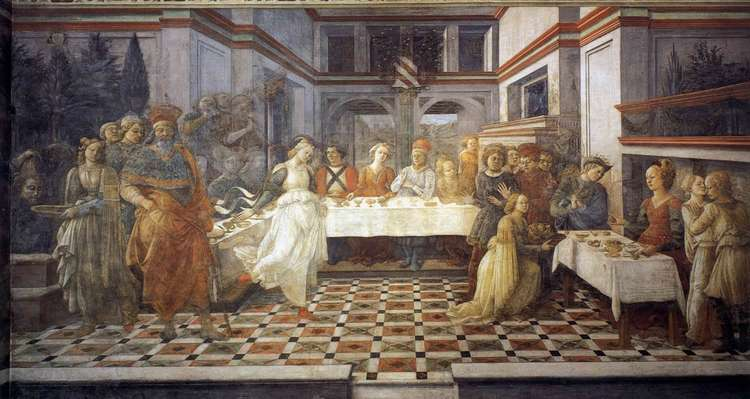
\includegraphics[width=\columnwidth]{img/lippi_feast_herod.jpg}
\caption{Filippo Lippi, ``The Feast of Herod: Salome's Dance.''
Fresco, Cappella Maggiore, Duomo, Prato, Italy, c.1460--1464.}%
\label{fig:lippi_feast_herod}
\end{figure}

\begin{figure}[h]
\centering
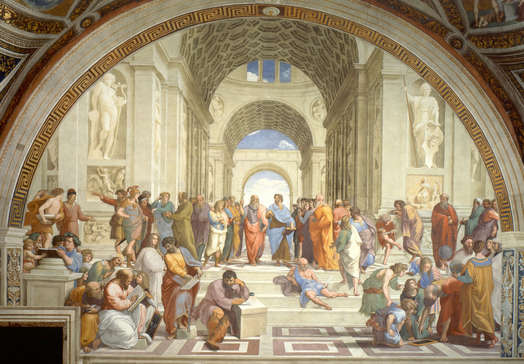
\includegraphics[width=\columnwidth]{img/raphael_school_athens.jpg}
\caption{Raphael, The School of Athens (1509)}%
\label{fig:raphael_school_athens}
\end{figure}

\begin{figure}[h]
\centering
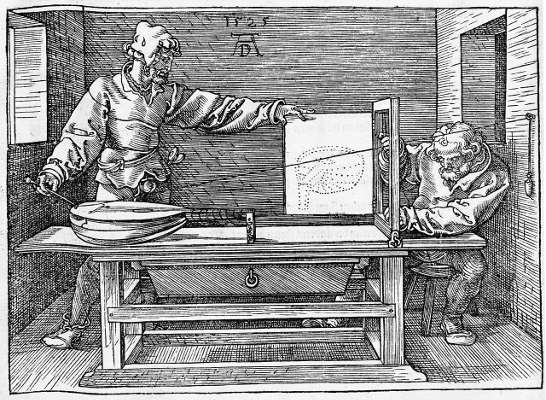
\includegraphics[width=\columnwidth]{img/durer_perspective_machine.jpg}
\caption{D\"urer's perspective machine (1525)}%
\label{fig:durer_perspective_machine}
\end{figure}

The study of the image formation process has a long history.
The earliest formulations of the geometry of image formation
can be traced back to \textbf{Euclid} (4th century B.C.).
Examples of a partially correct \textbf{perspective projection}
are visible in the \textbf{frescoes and mosaics of Pompeii} (1 B.C.).\\

These skills seem to have been lost with the fall of the Roman empire.
Correct perspective projection emerged again around 1000 years later
in early \textbf{Renaissance art}.\\

Among the proponents of perspective projection are the
Renaissance artists \textbf{Brunelleschi, Donatello} and \textbf{Alberti}.
The first treatise on the projection process, \textbf{``Della Pittura''},
was published by \textbf{Leon Battista Alberti}.\\

Appart from the geometry of image formation, the study of the
interaction of light with matter was propagated by artists like
\textbf{Leonardo da Vinci} in the 1500s and by Renaissance painters
such as \textbf{Caravaggio} and \textbf{Raphael}.\\

In Figure~\ref{fig:lippi_feast_herod} and Figure~\ref{fig:raphael_school_athens}
the perspective emerges from the vanishing point.

\begin{figure}[h]
\centering
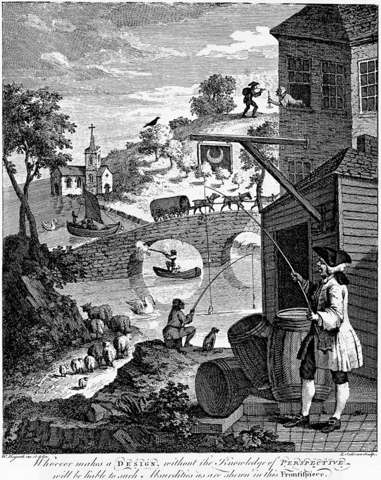
\includegraphics[width=\columnwidth]{img/hogarth_satire.jpg}
\caption{Satire by Hogarth 1753}%
\label{fig:hogarth_satire}
\end{figure}

\begin{figure}[h]
\centering
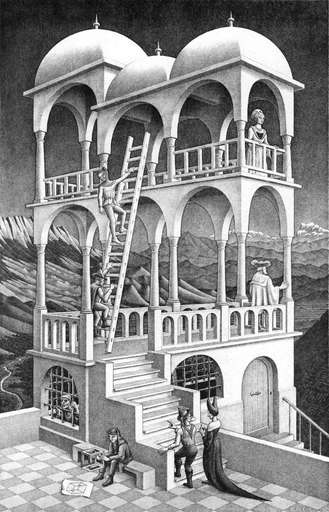
\includegraphics[width=\columnwidth]{img/escher_belvedere.jpg}
\caption{Escher, Belvedere 1958}%
\label{fig:escher_belvedere}
\end{figure}

D\"urer devised a machine to get a perspectively correct image,
see Figure~\ref{fig:durer_perspective_machine}.
It is a manual reproduction of what a camera does today.\\

Many artists played with those perspective rules to create images
that seems locally correct but have inconsitent depth or gravity, like
in Figures~[\ref{fig:hogarth_satire},\ref{fig:escher_belvedere}].


\subsection{Mathematical Representation}%
\label{sub:mathematical_representation}


\begin{figure}[h]
\centering
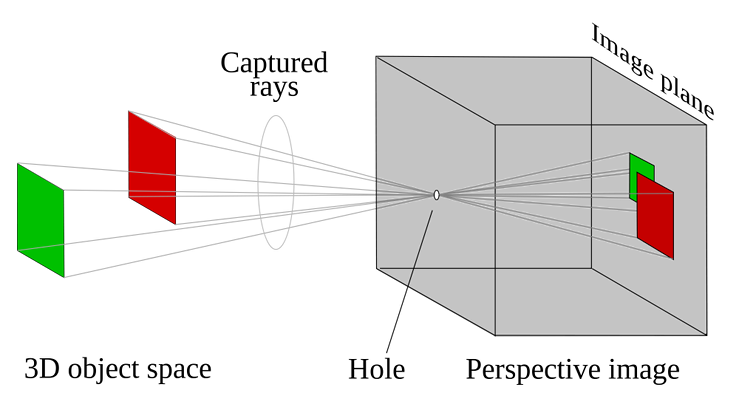
\includegraphics[width=\columnwidth]{img/pinhole_camera.png}
\caption{Pinhole camera model}%
\label{fig:pinhole_camera}
\end{figure}

\begin{figure}[h]
\centering
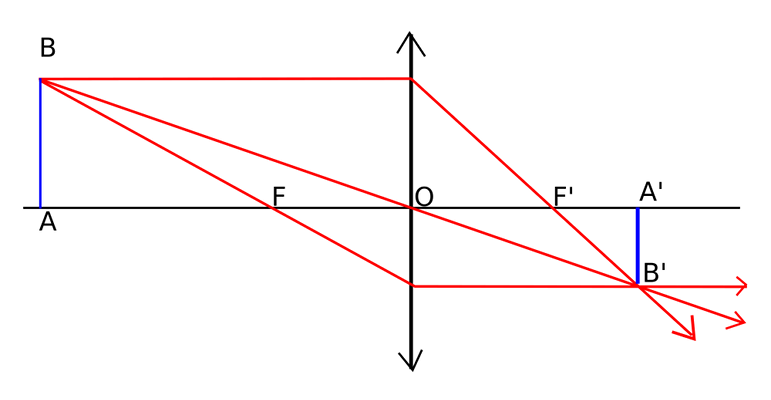
\includegraphics[width=\columnwidth]{img/convex_lense.png}
\caption{Thin convex lense model}%
\label{fig:convex_lense}
\end{figure}

Perspective projection emerges by the so-called pinhole camera model
(see Figure~\ref{fig:pinhole_camera}).
It's main issue is that the hole has to be very small,
perventing light to enter the capture device.
In order to augment the the amount of light we use lenses\\

As visible in (Figure~\ref{fig:convex_lense}), the image is upside down
in the image plan. In order to avoid dealing with minus signs in the
equations, we pretend that the image plan is virtually on the same
side than the object. The perspective thansformation $\pi$ is given by
\[ \pi : \R^3 \rightarrow \R^2; \quad
	\bm{X} \mapsto x = \pi(\bm{X}) =
	\begin{pmatrix}
		f \frac{X}{Z} \\
		f \frac{Y}{Z} \\
	\end{pmatrix}
\]
Where $f$ is the focal length, $X,Y,Z$ are the object coordinates
in the 3D world, the $z$ axis being the camera axis.
The one challenge we have to overcome, is that this transformation is non linear.\\

In order to do so, we will use \textbf{homogeneous coordinates},
which is basically similar to multiplying everything by $Z$:
\[ Z \bm{x} = Z \begin{pmatrix} x \\ y \\ 1 \end{pmatrix} =
	\begin{pmatrix}
		f & 0 & 0 & 0 \\
		0 & f & 0 & 0 \\
		0 & 0 & 1 & 0 \\
	\end{pmatrix}
	\begin{pmatrix}
		X \\ Y \\ Z \\ 1
	\end{pmatrix}
	= K_f \Pi_0 \bm{X}
\]
Where we have introduced the two matrices
\[K_f \equiv
	\begin{pmatrix}
		f & 0 & 0 \\
		0 & f & 0 \\
		0 & 0 & 1 \\
	\end{pmatrix}
	\quad \text{and} \quad
	\Pi_0 \equiv
	\begin{pmatrix}
		1 & 0 & 0 & 0 \\
		0 & 1 & 0 & 0 \\
		0 & 0 & 1 & 0 \\
	\end{pmatrix}
\]
The matrix $\Pi_0$ is referred to as the \textbf{standard projection matrix}.
A first order approximation can consider that all object points
are approximately at the same distance $\lambda > 0$. Thus we obtain:
\[\lambda \bm{x} = K_f \Pi_0 \bm{X}\]

We know that due to the \textbf{rigid motion of the camera},
the point $\bm{x}$ \textbf{in camera coordinates} is given as a function
of the point in \textbf{wold coordinates} $\bm{X}_0$ by:
\[\bm{X} = R \bm{X}_0 + T\]
or in homogeneous coordinates:
\[\bm{X} = g \bm{X}_0 = \begin{pmatrix}R & T \\ 0 & 1\end{pmatrix} \bm{X}_0\]
In total, the transformation from world coordinates to image coordinates
is therefore given by:
\[\boxed{\lambda\ \bm{x} = K_f\ \Pi_0\ g\ \bm{X}_0}\]


\subsection{Intrinsic Parameters}%
\label{sub:intrinsic_parameters}


If the camera is not centered at the optical center, we have an additional
translation $o_x, o_y$. The point were the optical axis intersects
the image plan is called the \textbf{principal point}.\\

If pixels do not have unit scale, we need to introduce
additional scaling factors $s_x$ and $s_y$.
If pixels are not rectangular, we also have a \textbf{skew factor} $s_{\theta}$.\\

The transformation from initial real world coordinates to final pixel coordinates
follows the following steps:
World (3D, $\bm{X}_0$) $\mapsto$ Camera (3D, $\bm{X}$)
$\mapsto$ Image (2D, $\bm{x}$) $\mapsto$ Pixel (2D, $\bm{x'}$).\\

The pixel coordinates $\bm{x'} = (x',y',1)$ are given by:
\[\lambda \begin{pmatrix}x' \\ y' \\ 1\end{pmatrix} =
	K_s\ K_f\ \Pi_0
	\begin{pmatrix}X \\ Y \\ Z \\ 1\end{pmatrix}
\]
where
\[K_s = \begin{pmatrix}
		s_x & s_{\theta} & o_x \\
		0 & s_y & o_y \\
		0 & 0 & 1 \\
	\end{pmatrix}
	\quad K_f =
	\begin{pmatrix}
		f & 0 & 0 \\
		0 & f & 0 \\
		0 & 0 & 1 \\
	\end{pmatrix}
\]
We call $K = K_s\ K_f$ the \textbf{intrinsic parameter matrix}.\\

Therefore, as a function of world coordinates, we have:
\[\boxed{ \lambda\ \bm{x'} = \Pi\ \bm{X}_0
	= K\ \Pi_0\ g\ \bm{X}_0}
\]
The $3 \times 4$ matrix $\Pi$ is called a \textbf{general projection matrix}.
If we get rid of $\lambda$ we obtain the following coordinates:
\[ x' = \frac{\tr{\pi_1} \bm{X}_0}{\tr{\pi_3} \bm{X}_0},\quad
 y' = \frac{\tr{\pi_2} \bm{X}_0}{\tr{\pi_3} \bm{X}_0},\quad
 z' = 1
\]
where $\tr{\pi_1}, \tr{\pi_2}, \tr{\pi_3} \in \R^4$
are the three rows of the projection matrix $\Pi$.


\subsection{Spherical Projection}%
\label{sub:spherical_projection}


The perspective pinhole camera introduced previously considers a planar
imaging suface. Instead, one can consider a spherical projection surface
given by the unit sphere
\[\mathbb{S}^2 \equiv \Set{x \in \R^3}{\|x\| = 1}\]
The \textbf{spherical projection} of a 3D point $\bm{X}$ is given by:
\[\pi_s : \R^3 \rightarrow \mathbb{S}^2;\quad
	\bm{X} \mapsto \bm{x} = \frac{\bm{X}}{\bm{|X|}}\]

The pixel coordinates $\bm{x}'$ as a function of the world coordinates
$\bm{X}_0$ are:
\[
	\lambda\ \bm{x}' = K\ \Pi_0\ g\ \bm{X}_0
\]
except that the scalar factor is now $\lambda = |\bm{X}|
= \sqrt{ X^2 + Y^2 + Z^2 }$.


\subsection{Radial Distortion}%
\label{sub:radial_distortion}


\begin{figure}[h]
\centering

\includegraphics[width=\columnwidth]{img/barrel_distortion.png}
\caption{Grid projection with radial distortion.}%
\label{fig:radial_distortion}
\end{figure}

The intrinsic parameters in the matrix $K$ model linear distortions
in the transformation to pixel coordinates.
In practice however, one can also encounter significant
\textbf{distortions along the radial axis}~[\ref{fig:radial_distortion}],
in particular in a wide field of view is used or if one uses cheaper cameras
such as webcams.
A simple effective model for such distortions is:
\[
	x = x_d ( 1 + a_1 r^2 + a_2 r^4 ),
	y = y_d ( 1 + a_1 r^2 + a_2 r^4 )
\]
where $\bm{x} \equiv (x_d, y_d)$ is the distorted point,
$r^2 = \|\bm{x}\|^2$.
Usually, $a_1$ and $a_2$ are estimated through a calibration step.\\

Other more sophisticated models exist (Devernay and Faugeras '95).
Parameters are computed from
\textbf{distortions of staight lines} (see Figure~\ref{fig:radial_distortion})
or \textbf{simultaneously with the 3D reconstruction}
(Zhang '96, Stein '97, Fitzgibbon '01).


\subsection{Preimage and Coimage}%
\label{sub:preimage_and_coimage}


Due to the unknown scale factor, each point is mapped not to a single
point $\bm{x}$, but to an \textbf{equivalence class of points} $\bm{ y \sim x}$.
It is therefore useful to \textbf{study ho lines are transformed}.
A line $L$ in 3-D is characterized by a base point
$\bm{X}_0 = \tr{(X_0, Y_0, Z_0, 1)} \in \R^4$ and a vector
$\bm{V} = \tr{(V_1, V_2, V_3, 0)} \in \R^4$ such that:
\[
	\bm{X} = \bm{X}_0 + \mu \bm{V}, \quad \mu \in \R
\]
The image of the line $L$ is given by:
\[
	\bm{x} \sim \Pi_0 \bm{X}
	= \Pi_0 ( \bm{X}_0 + \mu \bm{V} )
	= \Pi_0 \bm{X}_0 + \mu \Pi_0 \bm{V}
\]
All points $\bm{x}$ treated as vectors from the origin $o$ span a 2-D
subspace $P$. The intersection of this plane $P$ with the image plane
gives the image of the line.
$P$ is called the preimage of the line.
A \textbf{preimage of a point or a line} in the image plane
is the largest set of 3D points that give rise to an image
equal to the given point or line.\\

In case of points and lines, the preimage is a subspace of $\R^3$.
This subspace can also be represented by its orthogonal complement.
This complement is called the coimage.
The \textbf{coimage of a point or a line} is the subspace in $\R^3$
that is the (unique) orthogonal complement of its preimage.\\

\begin{tabular}{ll}
	image &$=$ preimage $\cap$ image plane,\\
	preimage &$=$ span (image),\\
	coimage &$=$ preimage$^{\bot}$,\\
\end{tabular}\\[1em]

In the case of a line $L$, the coimage can be characterized by
a vector $l$ such that:
\[
	\tr{l} \bm{x} = 0
\]
In summary we have the table~\ref{tab:expression_preimage_coimage}:

\begin{table}[h]
\small
\begin{tabular}{cccc}
	& Image & Preimage & Coimage \\ \midrule
	Point
		& $\text{span}(\bm{x}) \cap$ im.\,plane
		& $\text{span}(\bm{x})$
		& $\text{span}(\bm{\widehat{x}})$ \\
	Line
		& $\text{span}(\widehat{l}) \cap$ im.\,plane
		& $\text{span}(\widehat{l})$
		& $\text{span}(l)$ \\
\end{tabular}
\caption{Expression of preimage and coimage}%
\label{tab:expression_preimage_coimage}
\end{table}



\subsection{Projective Geometry}%
\label{sub:projective_geometry}


In order to formally write transformations by linear operations,
we made extensive use of \textbf{homogeneous coordinates} to represent
3D point as a 4D-vector $(X,Y,Z,1)$ with the last coordinate fixed to 1.
This normalization is not always necessary. One can represent 3D points
by a general 4D vector:
\[
	\bm{X} = (XW, YW, ZW, W)\ \in\ \R^4
\]
In general, an \textbf{n-dimensional projective space} $\mathbb{P}^n$
is the set of all one-dimensional subspaces (i.e.\ lines through the origin)
of the vector space $\R^{n+1}$.
A point $p \in \mathbb{P}^n$ can then be assigned homogeneous coordinates
$\bm{X} = \tr{(x_1, \ldots, x_{n+1})}$, among which at least one $x$ is nonzero.
For any nonzero $\lambda \in \R$, the coordinates
$\bm{Y} = \tr{(\lambda x_1, \ldots, \lambda x_{n+1})}$
represent the same point $p$.

\section{Estimating Point Correspondence}%
\label{sec:perspective_projection}


\subsection{From Photometry to Geometry}%
\label{sub:from_photometry_to_geometry}


In the last sections, we discussed how points and lines are transformed
from 3D world coordinates to 2D image and pixel coordinates.\\

In practice, \textbf{we do not actually observe points or lines,
but rather brightness or color values} at the individual pixels.
In order to transfer from this photometric representation to a
geometric representation of the scene, one can identify points with
\textbf{characteristic image features} and try to associate these
points with corresponding points in the other frames.\\

The matching of corresponding points will allow us to infer 3D structure.
Nevertheless, one should keep in mind taht this approach is suboptimal:
\textbf{by selecting a small number of feature points from each image,
we throw away a large amount of potentially useful information contained
in each image}.
Yet retaining all image information is computationally challenging.
The selection and matching of a small number of feature points,
on the other hand, was shown to permit tracking of 3D objects from
a moving camera in real time.

\begin{figure}[h]
	\centering
	
\includegraphics[width=\linewidth]{img/todo.png}
	\caption{Tracking of feature points}%
	\label{fig:traking_feature}
\end{figure}

To identify corresponding points in two or more images is one of the biggest
challenges in computer vision. Differences in point of view and
appearance can be challenging, due to materials, brightness, etc.
Small \textbf{baseline} make the tracking easier.\\

In what follows, we will assume that objects move rigidly.
In general, objects may also \textbf{deform non-rigidly}.
Moreover, there may be \textbf{partial occlusions}.
Quite often, points don't have correspondence in another image.
For example, in face tracking, teeth may disappear, smiles
may deform the face etc.\\

In point matching, one distinguishes two cases:

\begin{itemize}
	\item \textbf{Small deformation:} The deformation from one frame
		to the other is assumed to be (infinitesimally) small.
		In this case, the displacement from one frame to the othercan be estimated
		by classical \textbf{optic frow estimation}, for example using the methods
		of \textbf{Lucas/Kanade '81} or \textbf{Horn/Schunck '81}.
		These methods allow to model dense deformation fields (every pixel)
		but one can also track the displacement of a few feature points (faster).
	\item \textbf{Wide baseline stereo:} In this case the displacement is
		assumed to be large. A dense matching of all points to all is in general
		infeasible. Therefore, one typically selects a
		\textbf{small number of feature points} in each of the images
		and develops efficient methods to
		\textbf{find an appropriate pairing of points}.
\end{itemize}


\subsection{Small Deformation \& Optical Flow}%
\label{sub:small_deformation_optical_flow}


The transformation of all points of a rigidly moving objects is given by:
\[
	x_2 = h(x_1) = \frac{1}{\lambda_2(\bm{X})}
		(R \lambda_1(\bm{X}) x_1 + T)
\]
Locally this motion can be \textbf{approximated} in several ways.
\begin{itemize}
	\item Translation model: $h(x) = x + b$
	\item Affine model: $h(x) = Ax + b$
\end{itemize}
The 2D affine model can also be written with an offset $u$ as:
$h(x) = x + u(x)$ where:
\begin{align*}
	u(x) & = S(x)\ p \\
		 & = \begin{pmatrix}
				x & y & 1 & 0 & 0 & 0 \\
				0 & 0 & 0 & x & y & 1 \\
			\end{pmatrix}
			\tr{(p_1,p_2,p_3,p_4,p_5,p_6)}
\end{align*}

The \textbf{optic flow} refers to the apparent 2D motion field observable
between consecutive images of a video.
It is different from the motion of objects in the scene,
in the extreme case of motion along the camera axis, for example,
there is no optic frow, while on the other hand, camera rotation
generates an optic flow field event for entirely static scenes.\\

I 1981, two seminal works on optic flow estimation were published,
namely the works of \textbf{Lucas \& Kanade}, and of
\textbf{Horn \& Schunck}. Both methods have become very influential
with thousands of citations. They are complementary in the sense
that the Lucas-Kanade method generates, sparse flow vectors
under the assumption of constant motion in a local neighborhood,
whereas the Horn-Schunck method generates a dense flow field under
the assumption of spatially smooth flow fields.\\

Despite more than 30 years of research, the estimation of optic flow
fiels is still a highly active research direction.
Due to its simplicity, we will review the Lucas-Kanade method.


\subsection{The Lucas-Kanade Method}%
\label{sub:the_lucas_kanade_method}


\begin{itemize}
	\item \textbf{Brightness Constancy Assumption}:
		Let $x(t)$ denote a moving point at time $t$, and $I(x,t)$
		a video sequence, then:
		\[
			I(x(t),t) = \text{const.} \forall t,
		\]
		i.e.\ the brightness of point $x(t)$ is constant.
		Then the total time derivative must be zero:
		\[
			\frac{d}{dt} I(x(t),t)
			= \nabla \tr{I} \left(\frac{dx}{dt}\right)
				+ \frac{\partial I}{\partial t}
			= 0
		\]
		This constraint is often called the (differential)
		\textbf{optical flow constraint}. The desired local flow vector
		(velocity) is given by $v = \frac{dx}{dt}$.
		The fact that we can only recover the variation along
		the gradient is called in the literature,
		\textbf{the aperture problem}.

	\item \textbf{Constant motion in a neighborhood}:
		Since the above equation cannot be solved for $v$,
		one assumes that $v$ is constant over a neighborhood $W(x)$
		of the point $x$:
		\[
			\nabla \tr{I (x',t)} v + \frac{\partial I}{\partial t}(x',t)
				= 0,\quad \forall x'\ \in\ W(x)
		\]
		This assumption helps with the aperture problem.
\end{itemize}

The brightness is typically not exactly constant and the velocity
is typically not exactly the same for the local neighborhood.
\textbf{Lucas and Kanade (1981)} therefore compute the best velocity
vector $v$ for the point x by minimizing the \textbf{least squares error}.
\[
	E(v) = \int_{W(x)} | \nabla \tr{I(x',t)}v + I_t(x',t) | ^2 dx'
\]
Just a remark: nowadays, for precise optic flow computation,
one does not use this equation (not squared for example).
Expanding the terms and setting the derivative to zero one obtains:
\[
	\frac{dE}{dv} = 2 M v + 2 q = 0
\]
with
\[
	M = \int_{W(x)} \nabla I \tr{\nabla I} dx',\ \text{and} \
	q = \int_{W(x)} I_t \nabla I dx'
\]
If $M$ is invertible, then the solution is:
\[
	v = - \inv{M}q
\]
\begin{itemize}
	\item Translational motion: Lucas \& Kanade '81:
		\begin{align*}
			E(b) &= \int_{W(x)} | \tr{\nabla I} b + I_t |^2 dx' \\
			\frac{dE}{db} &= 0 \quad \implies b = \ldots
		\end{align*}
	\item Affine motion:
		\begin{align*}
			E(p) &= \int_{W(x)} | \tr{\nabla I(x')} S(x')p + I_t(x') |^2 dx' \\
			\frac{dE}{dp} &= 0 \quad \implies p = \ldots
		\end{align*}
		This energy $E(p)$ is quadratic in $p$ (a 6 parameters vector).
		We can essentially solve it doing the same as previously.
\end{itemize}

These techniques are easy to implement in theory.
However these should work only in the small deformation approximation (\roughly{} 1px).
This is very rarely the case with usual high resolution cameras.
One can use a \textbf{coarse to fine} algorithm to overcome this approximation.\\

In the formalism of Lucas and Kanade, one cannot always estimate a translational
motion. This problem is often referred to as the \textbf{aperture problem}.
It arises for example, if the region in the window $W(x)$ around the point $x$
has entirely constant intensity (for example a white wall),
because then $\nabla I(x) = 0$ and $I_t(x) = 0$ for all points in the window.\\

In order for the solution of $b$ to be unique, the \textbf{structure tensor}
\[
	M(x) = \int_{W(x)} \begin{pmatrix}
		I_x^2 & I_x I_y \\
		I_x I_y & I_y^2 \\
	\end{pmatrix} dx'
\]
needs to be invertible.
That means that we must have $\det M \neq 0$.
Or more realistically in practice, $M$ must not be \textbf{ill conditionned}.\\

If the structure tensor is not invertible but not zero,
then one can estimate the \textbf{normal motion} i.e.\ the motion
in direction of the image gradient.\\

In the regular case ($\det M \neq 0$), this leads to the following
simple feature tracker.
Feature tracking over a sequence of images can now be done as follows:
\begin{enumerate}
	\item For a given time instance $t$, compute at each point $x\in\Omega$
		the \textbf{structure tensor}
		\[
			M(x) = \int_{W(x)} \begin{pmatrix}
				I_x^2 & I_x I_y \\
				I_x I_y & I_y^2 \\
			\end{pmatrix} dx'
		\]
	\item Mark all points $x \in \Omega$ for which the determinant of $M$
		is larger than a threshold $\theta > 0$:
		\[
			\bm{\det M(x) \geq \theta}
		\]
	\item For all these points the local velocity is given by:
		\[
			\bm{b(x,t)} = - \inv{\bm{M(x)}} \begin{pmatrix}
				\int I_x I_t dx' \\
				\int I_y I_t dx' \\
			\end{pmatrix}
		\]
	\item Repeat the above steps for the points $x + b$ at time $t+1$.
\end{enumerate}


\subsection{Feature Point Extraction}%
\label{sub:feature_point_extraction}


\begin{figure}[h]
	\centering
	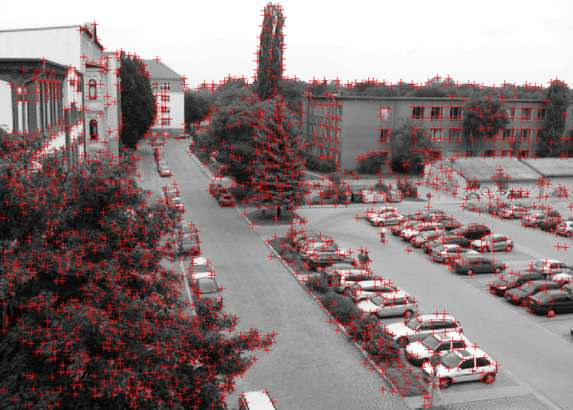
\includegraphics[width=\linewidth]{img/harris.jpg}
	\caption{Harris ``corner'' feature points.}%
	\label{fig:harris}
\end{figure}

Even $\det M(x) \neq 0$ does not guarantee robust estimates of velocity.
The inverse of $M(x)$ may not be very stable if, for example,
$M$ is ill conditionned (small determinant).\\

One of the classical feature detectors was proposed independently by
\textbf{F{\"o}rstner '84} and \textbf{Harris \& Stephens '88}
(Figure~\ref{fig:harris}). It is based on the \textbf{structure tensor}
\begin{align*}
	M(x) & \equiv G_{\sigma} * \nabla I \tr{\nabla I} \\
		& = \int G_{\sigma}(x-x') \begin{pmatrix}
			I_x^2 & I_x I_y \\
			I_x I_y & I_y^2 \\
		\end{pmatrix}
		(x') dx'
\end{align*}
where rather than simple summing over the window $W(x)$
we perform a summation weighted by a Gaussian $G$ of width $\sigma$.
The F\"orstner / Harris detector is given by:
\[
	\bm{C(x) = \det(M) + \kappa\ \text{trace}^2(M)}
\]
One selects points for which $C(x)>\theta$ with a threshold $\theta > 0$.


\subsection{Wide Baseline Matching}%
\label{sub:wide_baseline_matching}


Corresponding points and regions may look very different in different views.
In the case of \textbf{wide baseline matching}, large parts of the image
plane will not match at all because they are not visible in the other image.
In other words, while a given point may have many potential matches,
quite possibly it does not have any corresponding point in the other image.
Glass and in general, specular shiny objects really nasty to track.\\

One of the limitations of tracking features frame by frame is that
\textbf{small errors in the motion accumulate over time}
and the window gradually moves away from the point that was originally tracked.
This is known as \textbf{drift}.\\

A remedy is to match a given point back to the first frame.
This generally implies larger displacements between frames.
Two aspects matter when extending the above simple feature tracking
method to somewhat larger displacements:
\begin{itemize}
	\item Since the motion of the window between frames is
		(in general) no longer translational, one needs to
		\textbf{generalize the motion model} for the window $W(x)$,
		for example by using an \textbf{affine motion model}.
	\item Since the illumination will change over time
		(especially when comparing more distant frames), one can replace
		the sum-of-squared-differences by the
		\textbf{normalized cross correlation (NCC)} which is more
		\textbf{robust to illumination changes}.
\end{itemize}
\[
	NCC = \cos(v_1,v_2)
		= \frac{\inner{v_1}{v_2}}{|v_1|\ |v_2|}
\]
Where
\[
	v_i \equiv \text{vec}(I_i - \mean{I_i})
\]
$\mean{I_i}$ is the average intensity over the window $W(x)$.
By subtracting this average intensity, the measure becomes
\textbf{invariant to additive intensity changes} $I \rightarrow I + \gamma$.\\

Dividing by the intensity variances of each window makes the measure
\textbf{invariant to multiplicative changes} $I \rightarrow \gamma I$.\\

Let's look at the special case of \textbf{optimal affine transformation}.
The NCC can be used to determine the optimal affine transformation
between two given patches. Since the affine transformation is given
by $h(x) = A x + d$, we need to maximize the cross correlation
with respect to the $2\times2$-matrix $A$ and the displacement $d$:
\begin{align*}
	\widehat{A}, \widehat{d}
		& = \text{arg} \max_{A,d}\ NCC(A,D) \\
		& = \text{arg} \max_{A,d}\ \cos(v(x), v(Ax+d))
\end{align*}
This is not a convex cost function, so efficiently finding
appropriate optima is a challenge.\\

There exists many matching heuristics, some working better than others
depending on use cases. To evaluate the quality of point correspondence
algorithms, some have created \textbf{benchmarks}.
The challenge for creation of a good benchmark, is to get both
realistic images and accurate optic flow \textbf{ground truth}.
\begin{itemize}
	\item In the \textbf{Middlebury} benchmark, they superimposed
		very high frequency infrared pattern on images.
	\item In the \textbf{MPI Sintel} flow dataset is generated from
		an open source computer graphics short movie Sintel.
\end{itemize}

\section{Reconstruction from Two Views}%
\label{sec:reconstruction_two_views}


\subsection{The Reconstruction Problem}%
\label{sub:the_reconstruction_problem}


\begin{figure}[t]
	\centering
	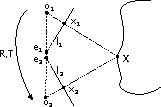
\includegraphics[width=\linewidth]{img/two-views.pdf}
	\caption{Camera motion and 3D structure from two views.}%
	\label{fig:two_views}
\end{figure}

In the last sections, we discussed how to identify point correspondences
between two consecutive frames. In this section,
we will tackle the next problem, namely that of
\textbf{reconstructing the 3D geometry of cameras and points}.
To this end, we will make the following assumptions:
\begin{itemize}
	\item We assume that we are given a
		\textbf{set of correspondences points} int two frames
		taken with the same camera from different vantage points.
	\item We assume that \textbf{the scene is static},
		i.e.\ none of the observed 3D points moved during the camera motion.
	\item We also assume that the
		\textbf{intrinsic camera (calibration) parameters are known}.
\end{itemize}

We will first estimate the \textbf{camera motion} from the set of
corresponding points. Once we know the relative location and
orientation of the cameras, we can reconstruct the 3D location
of all corresponding points by \textbf{triangulation}.\\

The projections of a point $X$ onto two images are denoted $x_1$ and $x_2$.
The optical centers of each camera are denoted by $o_1$ and $o_2$.
The intersections of the line $(o_1, o_2)$ with each image plane
are called the \textbf{epipoles} $\bm{e_1}$ and $\bm{e_2}$.
The intersections between the \textbf{epipolar plane $(\bm{o_1, o_2, X})$}
and the image planes are called \textbf{epipolar lines} $\bm{l_1}$ and $\bm{l_2}$.
There is an epipolar plane for each 3D point $X$.\\

In general 3D reconstruction is a challenging problem.
If we are given two views with 100 feature points in each of them,
then we have 200 point coordinates in 2D. The goal is to estimate
\begin{itemize}
	\item 6 parameters modeling the camera motion $R, T$
	\item $100 \times 3$ coordinates for the 3D points $X_i$
\end{itemize}
This could be done by minimizing the \textbf{projection error}:
\begin{align*}
	& E(R,T,X_1, \ldots, X_{100}) \\
	& = \sum_{j} \| x_1^j - \pi(X_j) \|^2 + \| x_2^j - \pi(R,T,X_j) \|^2
\end{align*}
This amounts to a \textbf{difficult optimization problem (not convex)} called
\textbf{bundle adjustment}. It turns out that there is a more elegant
solution which allows to entirely get rid of the 3D point coordinates.\\


\subsection{The Epipolar Constraint}%
\label{sub:the_epipolar_constraint}


We know that $x_1$ (in homogeneous coordinates) is the projection of a 3D point $X$.
Given known camera parameters ($K = 1$) and no rotation or translation
of the first camera, we merely have a projeciton with unknown depth $\lambda_1$.
From the first to the second frame we additionally have a camera
rotation and translation ($R,T$) followed by a projection.
This gives the equations:
\[
	\lambda_1 x_1 = X,
	\lambda_2 x_2 = RX + T
\]
Inserting the first equation into the second, we get:
\[
	\lambda_2 x_2 = R(\lambda_1 x_1) + T
\]
Now we remove the translation by multiplying with $\widehat{T}$:
\[
	\lambda_2 \widehat{T} x_2 = \lambda_1 \widehat{T} R x_1
\]
And projection onto $x_2$ gives the \textbf{epipolar constraint}:
\[
	\boxed{ 0 = \tr{x_2}\ \widehat{T}\ R\ x_1 }
\]
By doing all this, we have achieved to get rid of 3D coordinates.
Instead of initial constrained problem, we have a somewhat weaker,
but simpler constrained problem.
This can no longer be solved with 5 points only,
but it is much easier to solve.\\

The epipolar constraint porvides a
\textbf{relation between the 2D point coordinates} of a 3D point
in each of the two images \textbf{and the camera transformation parameters}.
The original 3D point coordinates have been removed. The matrix
\[
E = \widehat{T}R\quad \in \RR{3}{3}
\]
is called the \textbf{essential matrix}.
The \textbf{epipolar constraint} is also known as
\textbf{essential constraint} or \textbf{bilinear constraint}.
\textbf{Geometrically}, this constraint states that the three vectors
$o_1 X$, $o_2 o_1$ and $o_2 X$ form a plane, i.e.\ the triple product
of these vectors is zero.
In coordinates of the second frame, $Rx_1$ gives the direction of the
vector $o_1X$; $T$ gives the direction of $o_2 o_1$, and $x_2$
is proportional to the vector $o_2 X$ such that:
\[
	\text{volume} = \tr{x_2} (T \times Rx_1) = 0
\]

The space of all essential matrices is called the \textbf{essential space}:
\[
	\mathcal{E} \equiv \left\{ \widehat{T}R\ |\
		R \in SO(3), T \in \R^3 \right\}\ \subset \RR{3}{3}
\]
\begin{theorem}[Huang \& Faugeras, 1989 --- Characterization of the essential matrix]
	A nonzero matrix $E \in \RR{3}{3}$ is an essential matrix if and only if
	$E$ has a singular value decomposition: $(SVD)\ E = U \Sigma \tr{V}$ with
		\[
			\Sigma = \text{diag}\{ \sigma, \sigma, 0 \}
		\]
	for some $\sigma > 0$ and $U, V \in SO(3)$.
\end{theorem}
\begin{theorem}[Pose recovery from the essential matrix]
	There exists exactly two relative poses $(R,T)$ with $R \in SO(3)$
	and $T \in \R^3$ corresponding to an essential matrix $E \in \mathcal{E}$.
	For $E = U \Sigma \tr{V}$, we have:
	\begin{align*}
		(\widehat{T}_1, R_1) & =
			( U R_Z({\textstyle +\frac{\pi}{2}}) \Sigma \tr{U}
			,\ U \tr{R}_Z(+{\textstyle\frac{\pi}{2}}) \tr{V} ) \\
		(\widehat{T}_2, R_2) & =
			( U R_Z({\textstyle -\frac{\pi}{2}}) \Sigma \tr{U}
			,\ U \tr{R}_Z(-{\textstyle\frac{\pi}{2}}) \tr{V} )
	\end{align*}
	In general, only one of these gives meaningful (positive) depth.
\end{theorem}


\subsection{Eight-Point Algorithm}%
\label{sub:eight_point_algorithm}


We have seen that the 2D-coordinates of each 3D point
are coupled to the camera parameters $R$ and $T$ through an epipolar constraint.
In the following, we will derive a 3D reconstruction algorithm
which proceeds as follows:
\begin{itemize}
	\item \textbf{Recover the essential matrix $E$} from the epipolar
		constraints associated with a set of point pairs.
	\item \textbf{Extract the relative translation and rotation}
		from the essential matrix $E$.
\end{itemize}
In general, the matrix $E$ recovered from a set of epipolar constraints
will not be an essential matrix. One can resolve this problem in two ways:
\begin{enumerate}
	\item Recover some matrix $E \in \RR{3}{3}$ from the epipolar constraint
		and then project it onto the essential space.
	\item Optimize the epipolar constraints in the essential space.
\end{enumerate}
While the second approach is in principle more accurate,
it involves a nonlinear constrained optimization.
So we will pursue the first approach which is simpler and faster.\\

First we rewrite the epipolar constraint as a scalar product
in the elements of the matrix $E$ and the coordinates
of the points $x_1$ and $x_2$. Let
\[
	E^s = \tr{(e_{11}, e_{21}, e_{31}, e_{12}, e_{22}, e_{32}, e_{13}, e_{23}, e_{33})}
		\in \R^9
\]
be the vector of elements of $E$ and
\[
	a = \bm{x}_1 \otimes \bm{x}_2 \in \R^9
\]
the \textbf{Kronecker product} of the vectors $\bm{x}_i = (x_i, y_i, z_i)$.
Then the epipolar constraint can be written as:
\[
	\boxed{ \tr{\bm{x}_2} E\ \bm{x}_1 = \tr{a} E^s = 0 }
\]
For $n$ point pairs, we can combine this into the linear system:
\[
	\boxed{ \chi E^s = 0,\quad \text{with}\ \chi = \tr{(a^1, a^2, \ldots, a^n)} }
\]
We see that the vector of coefficients of the essential matrix $E$
defines the \textbf{null space of the matrix $\chi$}
In order for the above system to have a unique solution
(up to a scaling factor and ruling out the trivial solution $E = 0$),
the \textbf{rank of the matrix $\chi$ needs to be exactly 8}.
Therefore, we need at least 8 point pairs.\\

In certain \textbf{degenerate cases}, the solution for the essential matrix
is not unique even if we have 8 or more point pairs.
One such example is the case that all points lie on a line or on a plane.\\

Clearly, we will not be able to recover the sign of $E$.
Since with each $E$, there are two possible assignments of rotation $R$
and translation $T$, we therefore end up with four possible
solutions for rotation and translation.\\

The numerically estimated coefficients $E^s$ will in general fot correspond
to an essential matrix. One can resolve this problem by projecting
it back to the essential space.

\begin{theorem}[Projection onto essential space]
	Let $F \in \RR{3}{3}$ be an arbitrary matrix with SVD:
	\[
		F = U \text{diag} \{ \lambda_1, \lambda_2, \lambda_3 \} \tr{V}
		,\quad \lambda_1 \geq \lambda_2 \geq \lambda_3.
	\]
	Then the essential matrix $E$ which minimizes the Frobenius norm
	$\| F-E \|_f^2$, is given by:
	\[
		E = U \text{diag}\{ \sigma, \sigma, 0 \} \tr{V},\quad
		\text{with}\ \sigma = \frac{\lambda_1 + \lambda_2}{2}
	\]
\end{theorem}

\subsubsection*{Eight Point Algorithm (Longuet-Higgins '81) summary}%
\label{ssub:eight_point_algorithm}

Given a set of $n=8$ or more point pairs $\bm{x}_1^i, \bm{x}_2^i$:
\begin{enumerate}
	\item \textbf{Compute an approximation of the essential matrix}.
		Construct the matrix $\chi = \tr{(a^1, a^2, \ldots, a^n)}$
		where $a^i = \bm{x}_1^i \otimes \bm{x}_2^i$.
		Find the vector $E^s \in \R^9$ which minimizes $\|\chi E^s\|$
		as the ninth column of $V_{\chi}$ (smallest singular value) in the SVD
		$\chi = U_{\chi} \Sigma_{\chi} \tr{ V_{\chi} }$.
		Unstack $E^s$ into a $3 \times 3$-matrix $E$.

	\item \textbf{Project onto essential space.}
		Compute the SVD
		$E = U \text{diag} \{ \sigma_1, \sigma_2, \sigma_3 \} \tr{V}$.
		Since in the reconstruction, $E$ is only defined up to a scalar,
		we project $E$ onto the normalized essential space by replacing
		the singular values $\sigma_1, \sigma_2, \sigma_3$ with 1,1,0.

	\item \textbf{Recover the displacement from the essential matrix.}
		The four possible solutions for rotation and translation are:
		\begin{align*}
			R &= U \tr{R_Z} \left( {\textstyle \pm \frac{\pi}{2}} \right) \tr{V}, \\
			\widehat{T} &= U R_Z \left( {\textstyle \pm \frac{\pi}{2}} \right) \Sigma\ \tr{U},
		\end{align*}
		with a rotation by $\pm \frac{\pi}{2}$ around $z$:
		\[
			\tr{R_Z} \left( {\textstyle \pm \frac{\pi}{2}} \right)
				= \begin{pmatrix}
					0 & \pm 1 & 0 \\
					\mp 1 & 0 & 0 \\
					0 & 0 & 1
				\end{pmatrix}
		\]
\end{enumerate}


\subsubsection*{Do we need eight points?}%
\label{ssub:do_we_need_eight_points}


The above reasoning showed that we need at least eight points
in order for the matrix $\chi$ to have rank $8$ and therefore
guarantee a unique solution for $E$.
Yet one can take into account the special structure of $E$.
\textbf{The space of essential matrices is actually a five-dimensional space},
i.e.\ $E$ only has 5 (and not 9) degrees of freedom.\\

A simple way to \textbf{take into account the algebraic properties of $E$}
is to make use of the fact that $\det E = 0$.
If now we have only 7 point pairs, the null space of $\chi$ will have
(at least) Dimension 2, spanned by two vectors $E_1$ and $E_2$.
Then we can solve for $E$ by determining $\alpha$ such that:
\[
	\det E = \det (E_1 + \alpha E_2) = 0
\]
Along similar lines,
\textbf{Kruppa proved in 1913 that one needs only five point pairs to recover $(R,T)$.}
In the case of degenerate motion (for example planar or circular motion),
one can resolve the problem with even fewer point pairs.
Similarly, if parameters are provided by other sensors (rotation by IMU, etc.)
one can also resolve with fewer point pairs.


\subsubsection*{Limitations and Further Extensions}%
\label{ssub:limitations_and_further_extensions}


Among the four possible solutions for $R$ and $T$, there is generally
\textbf{only one meaningful one} (which assigns positive depth to all points).\\

\textbf{The algorithm fails if the translation is exactly 0},
since then $E = 0$ and nothing can be recovered.
Due to noise this typically does not happen.\\

In the case fo infinitesimal view point change, one can adapt the eight point
algorithm to the \textbf{continuous motion case}, where the epipolar constraint
is replaced by the \textbf{continuous epipolar constraint}.
Rather than recovering $(R,T)$ one recovers the linear and angular
velocity of the camera.\\

In the case of independently moving objects, one can generalize the epipolar constraint.
For two motions for example, we have either one of the other is 0:
\[
	( \tr{\bm{x}_2} E_1 \bm{x}_1 ) ( \tr{\bm{x}_2} E_2 \bm{x}_1 ) = 0
\]
with two essential matrices $E_1$ and $E_2$.
Given a sufficiently large number of point pairs, one can solve the respective
equations for multiple essential matrices using polynomial factorization.


\subsection{Structure Recontruction}%
\label{sub:structure_recontruction}


The linear eight-point algorithm allowed us to estimate the camera transformation
parameters $R$ and $T$ from a set of corresponding point pairs.
Yet, the essential matrix $E$ and hence the translation $T$ are
\textbf{only defined up to an arbitrary scale $\|E\| = \|T\| = \gamma \in \R^+$}.
After recovering $R$ and $T$, we therefore have for point $X^j$:
\[
	\lambda_2^j \bm{x}_2^j
		= \lambda_1^j R \bm{x}_1^j + \gamma T,
		\quad j = 1, \ldots, n
\]
with unknown scale parameters $\lambda_i^j$.
We can eliminate one of these scales by applying $\widehat{ \bm{x}_2^j }$:
\[
	\lambda_1^j \widehat{ \bm{x}_2^j }R \bm{x}_1^j
		+ \gamma \widehat{ \bm{x}_2^j }T
		= 0, \quad j = 1, \ldots, n
\]
This corresponds to \textbf{$n$ linear systems} of the form:
\[
	\left( \widehat{ \bm{x}_2^j }R \bm{x}_1^j
		,\ \widehat{ \bm{x}_2^j }T
	\right)
	\begin{pmatrix}
		\lambda_1^j \\ \gamma
	\end{pmatrix}
	= 0, \quad j = 1, \ldots, n
\]
Combining the parameters
$\lambda = \tr{(\lambda_1^1, \lambda_1^2, \ldots, \lambda_1^n, \gamma)} \in \R^{n+1}$,
we get the linear equation system:
\[
	\boxed{ M \lambda = 0 }
\]
with
\[
	M \equiv \left( \text{diag}(\widehat{\bm{x}_2^j} R \bm{x}_1^j)
	,\ \widehat{\bm{x}_2^j} T \right)
\]
In practice, we cannot find a solution that is exactly 0,
so we try to find $\lambda$ minimizing 
$\|M\lambda\|^2 = \tr{\lambda} \tr{M} M \lambda $ under that
$\| \lambda \| = 1$.
The linear least squares estimate for $\lambda$ is given by the eigenvector
corresponding to the smallest eigenvalue of $\tr{M}M$.
It is \textbf{only defined up to a global scale}. It reflects the
\textbf{ambiguity} that the camera has moved twice the distance,
the scene is twice larger and twice as far away.\\

This algorithm is considered \textbf{closed form} since it has an
analytic solution. But the line between analytic and numerical
solutions is often quite blurry since in practice,
eigenvalues are computed using numerical approaches at some point.


\subsection{Bundle Adjustment}%
\label{sub:bundle_adjustment}


The eight-point algorithm discussed before has several nice properties.
In particular, we found \textbf{closed-form solutions} to estimate the camera
parameters and the 3D structure, based on \textbf{singular value decomposition}.
However, if we have noisy data $\bm{\tilde{x}}_1, \bm{\tilde{x}}_2$
(correspondences not exact or even incorrect), then we have:
\begin{itemize}
	\item no guarantee that $R$ and $T$ are as close as possible
		to the true solution, some kind of robustness.
		This is mainly due to unstable eigenvalue estimation.
	\item no guarantee that we will get a consistent reconstruction.
\end{itemize}


\subsubsection*{Nonlinear Optimization Methods}%
\label{ssub:nonlinear_optimization_methods}


In order to take noise and statistical fluctuation into account,
one can revert to a \textbf{Bayesian formulation} and determine
the most likely camera transformation $R, T$ and `true'
2D coordinates $\bm{x}$ given the measured coordinates $\bm{\tilde{x}}$,
by performing a \textbf{maximum aposteriori estimate:}
\begin{align*}
	& \arg \max_{\bm{x}, R, T} \mathcal{P}(\bm{x}, R, T\ |\ \bm{\tilde{x}}) \\
	=\ & \arg \max_{\bm{x}, R, T} \mathcal{P}(\bm{\tilde{x}}\ |\ \bm{x}, R, T)
		\ \mathcal{P}(\bm{x}, R, T)
\end{align*}
This approach will however involve modeling probability densities $\mathcal{P}$
on the fairly complicated space $SO(3) \times \mathbb{S}^2$
of rotation and translation parameters, as $R \in SO(3)$ and $T \in \mathbb{S}^2$
(3D translation with unit length).\\

Alternatively, one can perform a \textbf{constrained optimization} by
minimizing a cost function (similarity to measurements):
\[
	\phi (\bm{x}, R, T) =
		\sum_{j=1}^{n} \sum_{i=1}^{2}
		\| \bm{\tilde{x}}_i^j - \bm{x}_i^j \|^2
\]
subject to (consistent geometry):
\begin{align*}
	\tr{{\bm{x}_2^j}} \widehat{T} R \bm{x}_1^j &= 0, \\
	\tr{{\bm{x}_1^j}} e_3 &= 1, \\
	\tr{{\bm{x}_2^j}} e_3 &= 1, \\
	\text{for all}\ j &= 1, \ldots, n
\end{align*}


\subsubsection*{Bundle Adjustment}%
\label{ssub:bundle_adjustment}

Interestingly, the unknown depth parameters $\lambda_i$ do not appear
in the above cost functions. The depth parameters appear directly
in the \textbf{unconstrained optimization problem}:
\[
	\sum_{j=1}^n
		\| \bm{\tilde{x}}_1^j - \pi_1 ( \bm{X}^j ) \|^2
		+ \| \bm{\tilde{x}}_2^j - \pi_2 ( \bm{X}^j ) \|^2
\]
where $\pi_i$ denote the projectinos onto the two images.
Expressed in coordinates of the first camera frame,
this is equal to the cost function:
\begin{align*}
	&\phi( \bm{x}_1, R, T, \lambda ) = \\
	&\sum_{j=1}^n
		\| \bm{\tilde{x}}_1^j - \bm{x}_1^j \|^2
		+ \| \bm{\tilde{x}}_2^j - \pi(R \lambda_1^j \bm{x}_1^j + T) \|^2
\end{align*}
This optimization procedure is known as \textbf{bundle adjustment}.
The constrained optimization and the unconstrained bundle adjustment
can be seen as
\textbf{different parameterizations of the same optimization objective}.


\subsubsection*{Degenerate Configurations}%
\label{ssub:degenerate_configurations}

The eight-point algorithm only provides unique solutions (up to a scalar factor)
if all 3D points are in a ``general position''.
This is no longer the case for certain \textbf{degenerate configurations},
for which all points lie on certain 2D surfaces which are called
\textbf{critical surfaces}.\\

Typically these critical surfaces are described by a quadratic equation
in the three point coordinates, such that they are referred to as
\textbf{quadratic surfaces}.\\

While most critical configurations do not actually arise in practice,
a specific degenerate configuration which does arise often is the case that
\textbf{all points lie on a 2D plane} (such as floors, table, walls, \ldots).\\

For the structure-from-motion problem in the context of points on a plane,
one can exploit additional constraints which leads to the so-called
\textbf{four-point algorithm}.


\subsection{Four-Point Algorithm}%
\label{sub:four_point_algorithm}


\subsubsection*{Planar Homographies}%
\label{ssub:planar_homographies}


Let us assume that all points lie on a plane. If $\bm{X}_1 \in \R^3$
denotes the point coordinates in the first frame, and these lie on a plane
with normal $N \in \mathbb{S}^2$, then we have:
\[
	\tr{N} \bm{X}_1 = d \quad \Leftrightarrow \quad
	\frac{1}{d} \tr{N} \bm{X}_1 = 1
\]
In the frame two, we therefore have the coordinates:
\begin{align*}
	\bm{X}_2
		&= R \bm{X}_1 + T \\
		&= R \bm{X}_1 + T \frac{1}{d} \tr{N} \bm{X}_1 \\
		&= \left( R + \frac{1}{d} T \tr{N} \right) \bm{X}_1 \\
		&\equiv H \bm{X}_1, \quad H \in \RR{3}{3}
\end{align*}
The matrix $H$ is called a \textbf{homography matrix}.
Inserting the 2D coordinates, we get:
\[
	\lambda_2 \bm{x}_2 = H \lambda_1 \bm{x}_1 \quad \Leftrightarrow \quad
	\boxed{ \bm{x}_2 \sim H \bm{x}_1 }
\]
Where $\sim$ means equality up to scaling.
This expression is called a \textbf{planar homography}.
$H$ depends on camera and plane parameters.


\subsubsection*{From Point Pairs to Homography}%
\label{ssub:from_point_pairs_to_homography}


By multiplying with $\widehat{\bm{x}_2}$ we can eliminate $\lambda_2$ and obtain:
\[
	\boxed{ \widehat{\bm{x}_2} H \bm{x}_1 = 0 }
\]
This equation is called the \textbf{planar epipolar constraint} or
\textbf{planar homography constraint}.
Again, we can cast this equation into the form:
\[
	\tr{\bm{a}} H^s = 0
\]
where we have stacked the elements of $H$ into a vector
\[
	H^s = (H_{11}, H_{21}, \ldots, H_{33}) \in \R^9
\]
and introduced the matrix
\[
	\bm{a} \equiv \bm{x}_1 \otimes \widehat{\bm{x}_2}\ \in \ \RR{9}{3}
\]
Since $\widehat{\bm{x}_2}$ is of rank 2, each point pair provides
two independent equations. That is why, in the general case,
we need four pairs instead of eight.


\subsubsection*{The Four Point Algorithm}%
\label{ssub:the_four_point_algorithm}

Let us now assume we have $n \geq 4$ pairs of corresponding 2D points
$\{ \bm{x}_1^j, \bm{x}_2^j \}, j= 1, \ldots, n$ in the two images.
Each point pair induces a matrix $\bm{a}^j$.
We intregrate these into a larger matrix
\[
	\chi \equiv \tr{( \bm{a}^1, \ldots, \bm{a}^n )}\ \in\ \RR{3n}{9}
\]
and obtain the system
\[
	\chi H^s = 0
\]
As in the case of the essential matrix,
\textbf{the homography matrix can be estimated up to a scale factor}.
This gives rise to the \textbf{four point algorithm}:
\begin{itemize}
	\item For the point pairs, compute the matrix $\chi$.
	\item Compute a solution $H^s$ for the above equation by singular
		value decomposition of $\chi$.
	\item Extract the motion parameters from the homography
		matrix $H = R + \frac{1}{d} T \tr{N}$.
\end{itemize}


\subsubsection*{General Comments}%
\label{ssub:general_comments}

Clearly, the derivation of the four-point algorithm is in close
analogy to that of the eight-point algorithm.\\

Rather than estimating the essential matrix $E$ on estimates the
homography matrix $H$ to derive $R$ and $T$.
In the four-point algorithm, the homography matrix is decomposed
into $R,N$ and $T/d$.
In other words, one can reconstruct the normal of the plane,
but the translation is only obtained in units of the offset $d$
of the plane and the origin.\\

The 3D structure of the points can then be computed in the same manner as before.
Since on uses the strong constraint that all points lie in a plane,
the four-point algorithm only requires four correspondences.\\

There exist numerous relations between the essential matrix $E = \widehat{T}R$
and the corresponding homography matrix $H = R + T \tr{u}$
with some $u \in \R^3$, in particular:
\[
	E = \widehat{T}H, \quad \tr{H} E + \tr{E} H = 0
\]


\subsection{The Uncalibrated Case}%
\label{sub:the_uncalibrated_case}


\subsubsection*{The Case of Uncalibrated Camera}%
\label{ssub:the_case_of_uncalibrated_camera}


The reconstruction algorithms introduced above all assume that the camera
is calibrated (K = 1). The general transformation from a 3D point to the
image is given by:
\[
	\lambda \bm{x}'\
		=\ K\, \Pi_0\, g\, \bm{X} \
		=\ (KR, KT) \bm{X}
\]
with the \textbf{intrinsic parameter matrix} or \textbf{calibration matrix}:
\[
	K = \begin{pmatrix}
		f s_x & s_{\theta} & o_x \\
		0     & f s_y & o_y \\
		0     & 0     & 1
	\end{pmatrix}
	\quad \in \RR{3}{3}
\]
The calibration matrix maps metric coordinates into image (pixel) coordinates,
using the focal length $f$, the optical center $(o_x, o_y)$,
the pixel size $(s_x, s_y)$ and a skew factor $s_{\theta}$.
If these parameters are known, then one can simply
\textbf{transform the pixel coordinates $\bm{x}'$ to normalized coordinates}
$\bm{x} = \inv{\bm{K}} \bm{x}'$
to obtain the representation used in the previous sections.
This amounts to centering the coordinates with respect to the optical center etc.


\subsubsection*{The Fundamental Matrix}%
\label{ssub:the_fundamental_matrix}

If the camera parameters $K$ cannot be estimated in a calibration procedure beforehand,
then one has to deal with \textbf{reconstruction from uncalibrated views}.\\

By transforming all image coordinates $\bm{x}'$ with the inverse calibration
matrix $\inv{K}$ into metric coordinates $x$, we obtain the
\textbf{epipolar constraint for uncalibrated cameras:}
\[
	\tr{\bm{x}_2} \widehat{T} R \bm{x}_1 = 0
	\quad \Leftrightarrow \quad
	\tr{{\bm{x'}_2}} K^{-\top} \widehat{T} R \inv{K} \bm{x'}_1 = 0
\]
which can be written as
\[
	\boxed{ \tr{{\bm{x'}_2}} F \bm{x'}_1 = 0 }
\]
with the \textbf{fundamental matrix} defined as:
\[
	F
		\quad \equiv \quad
		K^{-\top} \widehat{T} R \inv{K}
		\quad = \quad
		K^{-\top} E \inv{K}
\]
Since the invertible matrix $K$ does not affect the rank of this matrix,
we know that $F$ has an SVD $F = U \Sigma \tr{V}$ with
$\Sigma = \text{diag} ( \sigma_1, \sigma_2, 0 )$.
In fact, \textbf{any matrix of rank 2 can be a fundamental matrix}.


\subsubsection*{Limitations}%
\label{ssub:limitations}

While it is straight-forward to extend the eight-point algorithm,
such that one can extract a \textbf{fundamental matrix} from a set
of corresponding image points, it is less straight forward how to proceed from there.\\

Firstly, on cannot impose a strong constraint on the specific structure
of the fundamental matrix (apart from the fact that the last singular value is zero).\\

Secondly, for a given fundamental matrix $F$, there does not exist a finite
number of decompositions into extrinsic parameters $R,T$ and intrinsic
parameters $K$ (even apart from the global scale factor).\\

As a consequence, one can only determine so-called \textbf{projective reconstructions}
i.e.\ reconstructions of geometry and camera position which are defined
up to a so-called projective transformation.\\

As a solution, one typically choses a \textbf{canonical reconstruction}
from the family of possible reconstructions.


\end{document}
